%%%%%%%%%%%%%%%%%%%%%%%%%%%%%%%%%%%%%%%%%%%%%%%%%%%%%%%%%%%%%%%%%%%%%%%%%%%%%
%%%
%%% File: thesis.tex, version 1.9, May 2016
%%%
%%% =============================================
%%% This file contains a template that can be used with the package
%%% cs.sty and LaTeX2e to produce a thesis that meets the requirements
%%% of the Computer Science Department from the Technical University of Cluj-Napoca
%%%%%%%%%%%%%%%%%%%%%%%%%%%%%%%%%%%%%%%%%%%%%%%%%%%%%%%%%%%%%%%%%%%%%%%%%%%%%

\documentclass[12pt,a4paper,twoside]{report}         
\usepackage{cs}         
\usepackage{longtable}
\usepackage{times}
\usepackage{graphicx}
\usepackage{tikz}
\usepackage{latexsym}
\usepackage{amsmath,amsbsy}
\usepackage{amssymb}
\usepackage[matrix,arrow]{xy}
\usepackage[T1]{fontenc}
\usepackage{ae,aecompl}
\usepackage{romanian} %definitii pentru diacritice; 
\usepackage{amstext}
\usepackage{graphics}
\usepackage[T1]{fontenc}
\usepackage{ae,aecompl}
\usepackage{algorithm}
%\usepackage{algorithmic}
\usepackage{color}
\usepackage{color}
\usepackage{makecell}
\usepackage{eurosym}
\usepackage{pifont}% http://ctan.org/pkg/pifont
\usepackage{tabu}
\usepackage{xfp}
\usepackage{multirow}
\usepackage{enumitem}

% \mastersthesis
\diplomathesis
% \leftchapter
\centerchapter
% \rightchapter
\singlespace
% \oneandhalfspace
% \doublespace

\renewcommand{\thesisauthor}{Diana BEJAN}    %% Your name.
\renewcommand{\thesismonth}{Iulie}     %% Your month of graduation.
\renewcommand{\thesisyear}{2019}      %% Your year of graduation.
\renewcommand{\thesistitle}{BITSTORED \\SISTEM DE STOCARE SECURIZAT'A A FI'SIERELOR} % Title
\renewcommand{\thesissupervisor}{ Senior Lector Eng. Cosmina IVAN}
\newcommand{\department}{FACULTATEA DE AUTOMATIC'A 'SI CALCULATOARE\\
DEPARTAMENTUL CALCULATOARE}
\newcommand{\thesis}{LUCRARE DE LICEN'T'A}
\newcommand{\uline}[1]{\rule[0pt]{#1}{0.4pt}}
%\renewcommand{\thesisdedication}{P'arin'tilor mei}
\newcommand{\utcnlogo}{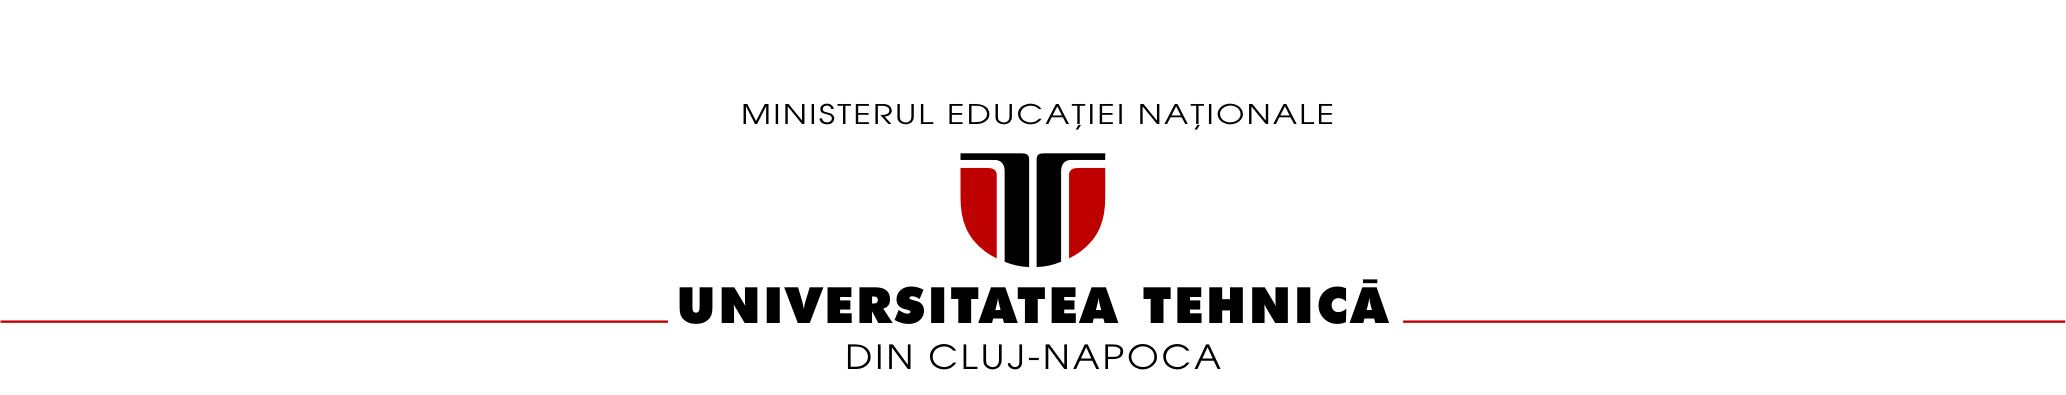
\includegraphics[width=15cm]{img/utcn.jpg}}
\newcommand{\greencheck}{\color{green}  \ding{51}}
\newcommand{\orangepm}{\color{orange} \textbf{$\pm$}}

\newcommand{\redxmark}{\color{red} \ding{55}}

\begin{document}
%\frontmatter
%\pagestyle{headings}

\newenvironment{definition}[1][Defini'tie.]{\begin{trivlist}
\item[\hskip \labelsep {\bfseries #1}]}{\end{trivlist}}



%\thesistitle                    %% Generate the title page.
%\authordeclarationpage                %% Generate the declaration page.





\begin{center}
%\includegraphics[width=15cm]{img/tucn.jpg}  
\utcnlogo

{\bf \department}

\vspace{4cm}

{\bf \thesistitle} %LICENSE THESIS TITLE}

\vspace{1.5cm}

\thesis

\vspace{6cm}

Absolvent: {\bf \thesisauthor} 

Conduc'ator 'stiin'tific: {\bf \thesissupervisor}

\vspace{3cm}
{\bf \thesisyear}
\end{center}

\thispagestyle{empty}
\newpage

\begin{center}
\utcnlogo

{\bf \department}
\end{center}
\vspace{0.5cm}

%\begin{small}
\begin{tabular}{p{7cm}p{8cm}}
 %\hspace{-1cm}& VIZAT,\\
 \hspace{-1cm}DECAN, & DIRECTOR DEPARTAMENT,\\
\hspace{-1cm}{\bf Prof. dr. ing. Liviu MICLEA} & {\bf Prof. dr. ing. Rodica POTOLEA}\\  
\end{tabular}
 
\vspace{2cm}

\begin{center}
Absolvent: {\bf \thesisauthor}

\vspace{1cm}

{\bf \thesistitle}
\end{center}

\vspace{1cm}

\begin{enumerate}
 \item {\bf Enun'tul temei:} Crearea unui sistem de stocare a fisierelor in cloud, acesta fiind disponibil sub forma de  mobile(IOS si Android) si  de aplica'tie web. Aplica'tia realizazeaz'a stocarea fi'sierelor 'in forma criptat'a, pentru a oferi protec'tie sporit'a a datelor, 'si compresat'a pentru utilizarea eficient'a a spa'tiului de stocare al utilizatorului. De asemenea sistemul ofer'a un mecanism de restabilire a datelor printr-un sistem de logare avansat.
\item {\bf Con'tinutul lucr'arii:} {Pagina de prezentare, Cuprins, Introducere, Obiectivele Proiectului, Studiu Bibliografic, Analiz'a 'si Fundamentare Teoretic'a, Proiectare de Detaliu 'si Implementare, Testare 'si Validare, Manual de Intalare 'si Utilizare, Concluzii ,Bibliografie, Anexe.}
\item {\bf Locul document'arii:} Universitatea Tehnic'a din Cluj-Napoca, Departamentul Calculatoare
\item {\bf Consultan'ti:} Senior Lector Eng. Cosmina Ivan
\item {\bf Data emiterii temei:} 1 ianuarie 2019
\item {\bf Data pred'arii:} 12 iulie 2019
  \end{enumerate}
\vspace{1.2cm}

\hspace{6cm} Absolvent: \uline{6cm} 

\vspace{0.5cm}
\hspace{6cm} Coordonator 'stiin'tific: \uline{5cm} 
%\end{small}

\thispagestyle{empty}


\newpage
$ $
%\begin{center}
%\utcnlogo

%{\bf \department}
%\end{center}

\thispagestyle{empty}
\newpage

\begin{center}
\utcnlogo

{\bf \department}
\end{center}

\vspace{0.5cm}

\begin{center}
{\bf
Declara'tie pe proprie r'aspundere privind\\ 
autenticitatea lucr'arii de licen't'a}
\end{center}
\vspace{1cm}



Subsemnatul(a) \\
\uline{14.8cm}, 
legitimat('a) cu \uline{4cm} seria \uline{3cm} nr. \uline{4cm}\\
CNP \uline{9cm}, autorul lucr'arii \uline{2.8cm}\\
\uline{16cm}\\
\uline{16cm}\\
elaborat'a 'in vederea sus'tinerii examenului de finalizare a studiilor de licen't'a la Facultatea de Automatic'a 'si Calculatoare, Specializarea \uline{7cm} din cadrul Universit'a'tii Tehnice din Cluj-Napoca, sesiunea \uline{4cm} a anului universitar \uline{3cm}, declar pe proprie r'aspundere, c'a aceast'a lucrare este rezultatul propriei activit'a'ti intelectuale, pe baza cercet'arilor mele 'si pe baza informa'tiilor ob'tinute din surse care au fost citate, 'in textul lucr'arii 'si 'in bibliografie.

Declar, c'a aceast'a lucrare nu con'tine por'tiuni plagiate, iar sursele bibliografice au fost folosite cu respectarea legisla'tiei rom\ia ne 'si a conven'tiilor interna'tionale privind drepturile de autor.

Declar, de asemenea, c'a aceast'a lucrare nu a mai fost prezentat'a 'in fa'ta unei alte comisii de examen de licen't'a.

'In cazul constat'arii ulterioare a unor declara'tii false, voi suporta sanc'tiunile administrative, respectiv, \emph{anularea examenului de licen't'a}.

\vspace{1.5cm}

Data \hspace{8cm} Nume, Prenume

\vspace{0.5cm}

\uline{3cm} \hspace{5cm} \uline{5cm}

\vspace{1cm}
\hspace{9.4cm}Semn'atura

\thispagestyle{empty}

\newpage


%\listoftables
%\listoffigures

%\clearpage 
%\newpage

%\begin{comment}
{\color{red}{\bf De citit 'inainte} (aceast'a pagin'a se va elimina din versiunea final'a)}:
\begin{enumerate}
 \item Cele trei pagini anterioare (foaie de cap'at, foaie sumar, declara'tie) se vor lista pe foi separate (nu fa't'a-verso), fiind incluse 'in lucrarea listat'a. 
 Foaia de sumar (a doua) necesit'a semn'atura absolventului, respectiv a coordonatorului.
 Pe declara'tie se trece data c\ia nd se pred'a lucrarea la secretarii de comisie.
 \item Pe foaia de cap'at, se va trece corect titulatura cadrului didactic 'indrum'ator, 'in englez'a (consulta'ti pagina de unde a'ti desc'arcat acest document pentru lista cadrelor didactice cu titulaturile lor).
 \item Documentul curent {\bf nu} a fost creat 'in MS Office. E posibil sa fie mici diferen'te de formatare. 
\item Cuprinsul 'incepe pe pagina nou'a, impar'a (dac'a se face listare fa't'a-verso), prima pagin'a din capitolul Introducere tot a'sa, fiind numerotat'a cu 1. % Pentru actualizarea cuprinsului, click dreapta pe cuprins (zona cuprinsului va apare cu gri), Update field-$>$Update entire table.
\item Vizualiza'ti (recomandabil 'si 'in timpul edit'arii) acest document % după ce activaţi vizualizarea simbolurilor ascunse de formatare (apăsaţi simbolul  din Home/Paragraph).
\item Fiecare capitol 'incepe pe pagin'a nou'a. % datorită simbolului ascuns Section Break (Next Page) care este deja introdus la capitolul precedent. Dacă ştergeţi din greşeală simbolul, se reintroduce (Page Layout -> Breaks).
\item Folosi'ti stilurile predefinite (Headings, Figure, Table, Normal, etc.)
\item Marginile la pagini nu se modific'a.
\item Respecta'ti restul instruc'tiunilor din fiecare capitol.
\end{enumerate}
 
%\end{comment}

\newpage
\pagenumbering{arabic}
\setcounter{page}{1}
\tableofcontents
\newpage



\chapter{Introducere - Contextul proiectului}
\pagestyle{headings}
'In epoca contemporan'a se observ'a o tendin't'a continu'a a digitaliz'arii si transform'arii digitale, fapt care aduce un impact enorm atât asupra marilor companii, atât 'si asupra utilizatorilor individuali. Lumea bazat'a pe date va fi permanent'a, mereu 'in urm'arire, mereu 'in stadiu de monitorizare - pentru c'a va fi mereu 'in stadiu de 'inv'a'tare.

IDC\cite{IDCdigitization}  a definit trei loca'tii principale 'in care digitalizarea are loc 'si unde este creat con'tinutul de date: tip nucleu (centre de date tradi'tionale si de tip cloud), tip muchie (infrastructuri de tip sucursal'a), 'si obiectivele finale (PC-uri, telefoane si dispozitive IoT). Sumarizarea tuturor acestor date, 'in momentul 'in care sunt  create, capturate sau replicate, se nume'ste Global Datasphere, 'si aceasta se confrunt'a cu o cre'stere spectaculoas'a. IDC (International Data Corporation) estimeaz'a c'a volumul de date din Global Datasphere va cre'ste de la 33 Zettabytes\footnote{1 Zetta byte echivalent cu $2^{70}$ bytes} 'in 2018 pân'a la 175 Zettabytes in 2025, evolu'tia se poate observa 'in Figura \ref{data_grow}.

\begin{figure}[H]
\begin{center}
\advance\leftskip-3cm
\advance\rightskip-3cm
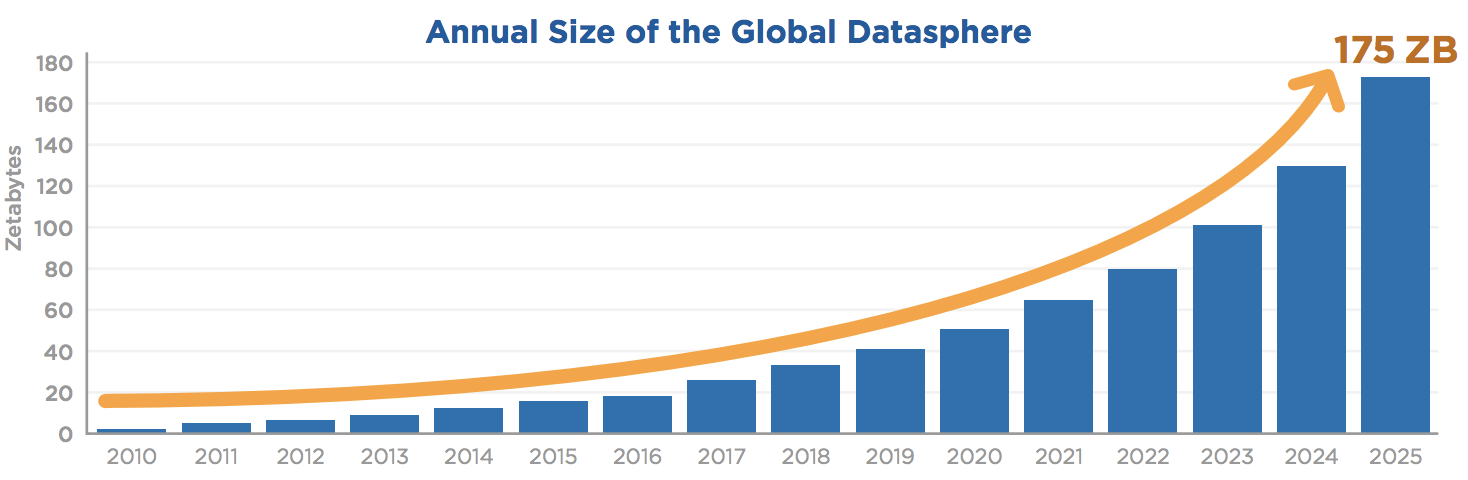
\includegraphics[keepaspectratio=true,scale=0.55]{img/data_grow.png}
\caption{Cre'sterea volumului de date 2010-2025}
\label{data_grow}
\end{center}
\end{figure}

'In trecutul recent utilizatorii erau responsabili pentru datele lor, 'insa dependen'ta 'si 'increderea lor 'in servciile cloud, 'in special din  cauza conectivit'a'tii, performan'tei si confortului, continua sa creasc'a ceea ce duce la noi provoc'ari pentru furnizorii de servicii cloud. Mediul afarcerilor urm'are'ste centralizarea managementului datelor, pentru a putea oferi securitate, analiz'a de date, experien't'a utilizator mai bun'a (prin comunicare 'intre dispozitive, IoT, personalizarea profilului). Responsabilitatea pentru managementul datelor utilizatorilor 'si businessurilor duce la o crestere continu'a a centrelor de date ale furnizorilor de servicii Cloud. Ca rezultat importan'ta serviciilor cloud cre'ste considerabil, iar utilizatorii nu doar permit acest lucru si se a'steapt'a la o crestere cât mai spectaculoas'a.

Volumul de date cât mai mare stocat 'in cloud este scopul industriei de stocare a datelor.
Pentru a supravie'tui 'intr-o lume care tinde  a fi condus'a de inteligen'ta artificial'a 'si sistemel autonome sistemele de cloud au nevoie s'a se perfec'tioneze tot mai mult pentru a 'tine pasul cu evolu'tia lumii.

'In calitate de clien'ti, oamenii doresc s'a ob'tin'a acces rapid 'si simplu la datele lor indiferent de or'a 'si loca'tia 'in care se afl'a. Sistemele cloud sunt provocate s'a ofere servicii performante de acces, care nu vor expune datele utilizatorilor. 

Organiza'tiile 'si utilizatorii au 'inceput s'a 'i'si schimbe destina'tia datelor de la infrastructuri fizice spre \textit{cloud}-ul public, al'tii 'ins'a au ínceput sa 'isi dezvolte propriile solu'tii de stocare, astfel profitând de toate beneficiile \textit{cloud}-ului. 'Ins'a securitatea datelor r'amâne cea mai mare problem'a, mai ales din cauza lipsei de control asupra infrastructurii fizice\cite{cloudsecurityautomation}. Toate sistemele 'incerc'a s'a se bazeze pe modelul CIA\footnote{Confidentiality, Integrity, and Availability}, acest sistem este prezentat 'in figura \ref{cia_sist}.
\begin{figure}[H]
\begin{center}
\advance\leftskip-3cm
\advance\rightskip-3cm
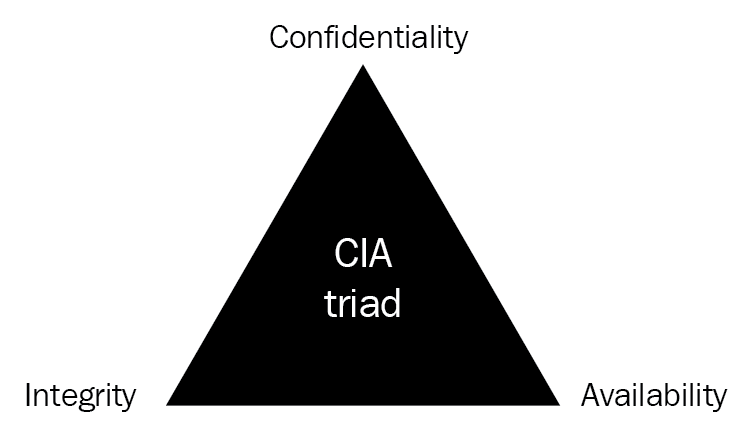
\includegraphics[keepaspectratio=true,scale=0.38]{img/cia_triad.png}
\caption{Triada CIA}
\label{cia_sist}
\end{center}
\end{figure}
Confiden'tialitatea se refer'a la protejarea datelor de la un access neautorizat. Integritatea se refer'a la protec'tia datelor de la modific'ari neautizate, orice modificare poate 'insemna o pierdere considerabil'a pentru utilizator sau organiza'tie. Disponibilitatea denot'a faptul c'a informa'tiile vor fi accesibile doar pentru utilizatorii care au drept de acces, o 'inc'alcare a acestei reguli, din nou, se va provoca pierderea unor date. Toate cele 3 aspecte sunt esen'tiale pentru securitatea datelor, 'ins'a acestea sunt uneori complicat de oferit.

Securitatea datelor este o problem'a foarte mare cu care se lupt'a zilnic dezvoltatorii de servicii \textit{cloud}. Multe din probleme se datoreaz'a expunerii nivelului de stocare, datele ar trebui s'a fie stocate 'in medii securizate, care ofer'a criptare eficient'a. Aceste problemepot fi 'inl'aturate doar prin indeplinirea strict'a a unor tratate de securitate avansat'a.

Cre'sterea volumului de date, pe de alt'a parte duce 'si la cre'sterea volumului fizic de \textit{hardware} necesar. Compresia datelor este o opera'tie care permite stocarea aceluia'si volum de date la un pre't mult mai redus\cite{data_compression_ibm}. Datorit'a compresiei un utilizator poate stoca un volum mai mare de date decât ii permite teoretic \textit{hardware}-ul. Pe lânga faptul c'a se reduce spa'tiul de stocare a datelor, compresia contribuie 'si la mic'sorarea timpului necesar pentru transmisie sau pentru opera'tiile I/E\cite{compression_adv}. 

Un alt beneficiu al compresiei este cre'sterea nivelului de securitate. Acest fapt se datoreaz'a alter'arii datelor, astfel chiar 'si un algoritm de criptare primitiv devine mult mai complicat de spart prin for't'a brut'a, 'in ecua'tie se mai adaug'a 'si decompresia datelor, care este o opera'tie costisitoare, nu se mai pot determina asocieri 'intre simboluri, 'intre secven'te de caractere 'si cuvintele dintr-o limb'a. Cu toate c'a se adaug'a un timp mare de procesare, 'in cazul unor date sensibile, aceast'a 'intârziere este una motivat'a din punctul de vedere al securit'a'tii datelor.

Cre'sterea 'increderii 'in sistemele de stocare, cre'sterea volumului de date, inclusiv 'si a celor de sensibilitate 'inalt'a, 'si  a num'arului de atacuri cibernetice creaz'a o nou'a provocare pentru sistemele de stocare cloud existente: cre'sterea securit'a'tii datelor. De asemenea acest aspect creaz'a 'si oportunit'a'ti noi pentru sistemele la 'inceput de drum, le ofer'a o pia't'a de defacere enorm'a 'si un num'ar ridicat de clien'ti care sunt gata s'a pl'ateasc'a preturi relativ ridicate pentru securitatea datelor sale.

Volumul de date cre'ste, 'ins'a pe lâng'a conceptul celor \textit{trei V}: volum, varietate 'si velocitate, se mai adaug'a 'si al 4-lea V: valoare. Pentru oferirea securit'a'tii datelor, anual se cheltuie 'in jur de \$100 miliarde, 'in 2019 aceast'a sum'a a ajuns la \$124 miliarde.

Aten'tia industriei IT ar trebui s'a se concentreze 'in jurul securit'a'tii cibernetice, cu referire mai mult la valoarea datelor, nu la volumul sau sursa lor. Solu'tiile sunt 'si trebuie s'a fie conduse de viziunea 'si gândirea oamenilor, dar validarea solu'tiilor ar trebui s'a fie validate de inteligen'ta datelor. 
 
Aceste fapte sunt un avantaj competitiv pentru indrustria IT 'si sunt o provocare pentru construirea unei culturi s'an'atoase a datelor.


\chapter{Obiectivele Proiectului}
'In acest capitol este prezentat'a tema proiectului, obiectivele 'si cerin'tele func'tionale esen'tiale  ale proiectului.
\section{Formularea temei}
Prin acest poroiect, se urm'are'ste implementarea unei platforme de \textit{Cloud Storage}, aceasta trebuie s'a ofere o bun'a protec'tie a datelor, aceste date s'a nu fie accesibile dezvoltatorilor sistemului, atacatorilor sau oric'arei alte institu'tii care colecteaz'a date. Sistemul este menit pentru stocarea datelor sensibile, sub r'aspunderea direct'a a utilizatorilor, de asemenea sistemul poate fi privit ca o platform'a f'ar'a cuno'stin'te despre datele stocate, nimeni altul decât proprietarul fi'sierelor nu poate decripta datele.

Conceptul sistemului este bazat pe arhitectura clasic'a \textit{client-server}, aceasta este prezentat'a 'in figura \ref{client_server}.

\begin{figure}[H]
\begin{center}
\advance\leftskip-3cm
\advance\rightskip-3cm
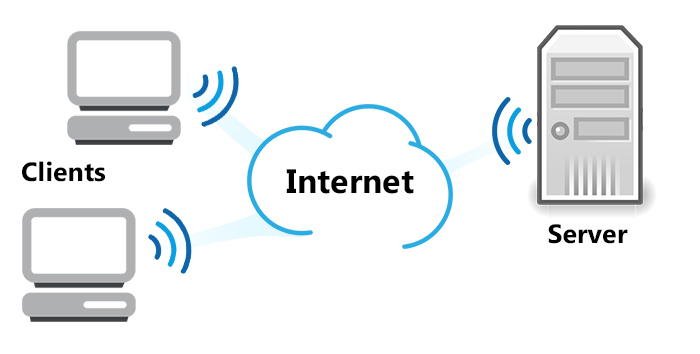
\includegraphics[keepaspectratio=true,scale=0.3]{img/client-server.jpeg}
\caption{Arhitectura Client-Server}
\label{client_server}
\end{center}
\end{figure}

Serverul la rândul s'au având o arhitectur'a bazat'a pe microservicii, fiecare mcroserviciu fiind organizat sub form'a de \textit{layer}. La nivel de aplica'tie, responsabilit'a'tile sunt parti'tionate 'intre server 'si client. La nivelul serverului, func'tionalit'a'tile esen'tiale sunt repartizate 'intre servicii, astfel fiind respectat principiul \textbf{Single-responsability} din SOLID\cite{solid}.
La nivel de microserviciu func'tionalit'a'tile sunt divizate la nivel de \textit{layer} 'si func'tie.

Serverul se ocup'a de prelucrarea 'si stocarea datelor. Func'tionalit'a'tile cheie sunt: compresie, criptare, conversie, steganografie, monitorizare 'si stocare. Partea de stocare a datelor este 'imp'ar'tit'a 'in 2: fi'siere 'si date personale. Datele utilizator sunt stocate 'iin MongoDB, iar cele despre fi'siiere in Couchbase, este imposibil s'a asociezi un fi'sier cu identiitatea unui utilizator f'ar'a accesul la ambele baze de date.

Aplica'tia  va trebui s'a fie proictat'a  astfel 'incât s'a poat'a satisface cereri de la sute sau mii de utilizatori concomitent, f'ar'a a implica 'intârzieri mari de r'aspuns. Apliica'tia va trebui s'a fie rezisten't'a la un nivel mare de utilizare 'si s'a se autoscaleze prin crearea unor replici ale aceluia'si cod, doar pentru microserviciile utilizate intens.

Sistemul va oferi utilizatorilor func'tionalit'a'tile de baz'a a unui sistem de stocare 'in \textit{cloud}: 'inc'arcare fi'sier, desc'arcare fi'sier, creare fi'sier nou, grupare fi'siere 'si management fi'siere. Pe lâng'a func'tionalit'a'tile enumerate, sistemul va oferi un nivel de securitate 'inalt prin criptarea tuturor datelor 'si eficien't'a de utilizare a spa'tiului prin compresia datelor. Cheia de criptare/decriptare nu va fi stocat'a nic'aieri 'in server sau client, utilizatorul va ave 'in totalitate responsabilitatea de a 'isi p'astra fi'sierele sigure 'si de a putea recupera datele stocate 'iin sistem, din p'acate este imposibil s'a i se ofere asisiten't'a 'in cazul pierderii parolei, regenerarea ei priin for't'a brut'a ar putea dura 'intre câteva ore 'si câ'tiva ani.

De asemenea la desc'arcarea unui fi'sier, utilizatorul va avea posibilitatea de a ascunde mesaje 'in imagini, sau de a aplica marcaje vizibile pe imagini. Aceast'a func'tionalitate poate fi folosit'a atunci când se partajeaz'a un fi'sier, pentru a determina dac'a datele au fost expuse diin sistem 'si identiitatea celui care le-a expus. Un exemplu de steganografie pe imagini este prezentat 'in figura \ref{stegano_example}.
\begin{figure}[H]
\begin{center}
\advance\leftskip-3cm
\advance\rightskip-3cm
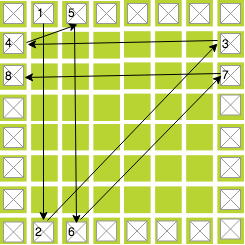
\includegraphics[keepaspectratio=true,scale=0.4]{img/stegano_example.png}
\caption{Exemplu de steganografie pe imagini}
\label{stegano_example}
\end{center}
\end{figure}
Dup'a cum se poate observa, manipularea bi'tilor nu este vizibil'a pentru ochiul uman, 'ins'a pentru calculator poate con'tine informa'tii valoroase.

Pentru client, se urm'are'ste implementarea unei aplica'tii web. Aceasta va trebui s'a interac'tioneze cu utilizatorii prin interfa'ta web 'si cu serverul prin apeluri de tip gRPC, pentru a asigura o vitez'a mai bun'a de transmisie 'si r'aspuns. Clientului nu 'ii vor fi cunoscute decât 3 dintre serviciile existente: serviciul de autentificare, servicul de management utilizatori 'si  serviciiul de management fi'siere.
\section{Obiectivele proiectului}
\begin{itemize}

\item[•]{Sistemul va oferi utilizatorilor experien'ta deplin'a a unui sistem de stocare 'in \textit{Cloud}: 'inc'arcare fi'sier, desc'arcare fi'sier, modificare fi'sier, grupare fi'siere.}

\item[•]{Sistemul va oferi utilizatorilor un nivel 'inalt de securitate a datelor personale prin folosirea unor algoritmi de criptare eficien'ti. Cheile nu vor fi stocate 'in sistem, iar datele vor fi aproape imposibil de decriptat de c'atre atacatori.}

\item[•]{Conexiunea 'intre client 'si server va fi securizat'a utilizând protocolul \textbf{HTTPS}. Astfel se va asigura c'a datele transmise vor fi protejate 'impotriva atcurilor de tipul \textit{man-in-the-middle}.}

\item[•]{Folosirea spa'tiiului de stocare va fi eficientiza'ta prin folosirea unor algoritmii de compresie eficien'ti, care permit reducerea volumului de date de maii mult de 2 ori 'in cazul unor date uzuale.}
\end{itemize}

\section{Cerin'te}
'In aceast'a sec'tiune sunt descrise 'si enumerate cerin'tele principale ale sstemului. Acestea se refer'a atât la func'tionalit'a'tile propriu-zise, cât 'si la experien'ta utilizatorului.
\subsection{Cerin'te func'tionale}
Cerin'tele func'tionale definesc func'tiile sistemului sau comportamentul s'au, unde func'tiile sunt descrise ca o specifica'tie sau set de ac'tiuni dintre intrare 'si ie'sire. Pornind de la
obiectivele proiectului, pot fi determinate urm'atoarele cerin'te func'tionale:

\begin{enumerate}[label=CF\arabic*]
\item{Ca utilizator ne'inregistrat, doresc s'a 'imi pot crea un cont nou.}
\item{Ca utilizator, doresc s'a m'a autentific 'in sistem utilizând numele de utilizator 'si parola, care au fost indicate la momentul 'inregistr'arii.}
\item{Ca Utilizator, doresc ca sesiunea mea s'a fie p'astrat'a 'si dup'a 'inchiderea \textit{browser}-ului.}
\item{Ca utilizator, dorec s'a 'imi opresc sesiunea curent'a prin deautentificare.}
\item{Ca utilizator, dorec s'a am posibilitatea de a 'imi bloca temporar contul, f'ar'a a pierde accesul la date.}
\item{Ca utilizator, dorec s'a am posibilitatea de a 'imi debloca contul.}
\item{Ca utilizator, dorec s'a am posibilitatea de a 'im sterge contul 'si toate datele stocate.}
\item{Ca utilizator, doresc s'a pot modifica datele mele de utilizator, cum ar fi parola, nume, poz'a de profil.}
\item{Ca utilizator, doresc s'a pot primi o confirmare a 'inregistr'arii pe mail-ul indicat la momentul 'inregistr'arii 'in sistem.}
\item{Ca utilizator, doresc s'a pot vizualiza profilul meu.}
\item{Ca utilizator, doresc s'a pot vizualiza fi'sierele mele din \textit{Drive} 'si s'a pot naviga prin ierarhia de directoare.}
\item{Ca utilizator, doresc s'a pot crea un fi'sier nou, care s'a aib'a sau nu con'tinut.}
\item{Ca utilizator, doresc s'a pot crea un director nou.}
\item{Ca utilizator, doresc s'a pot 'incarca un fi'sier 'in sistem.}
\item{Ca utilizator, doresc s'a pot modifica un fi'sier care se afl'a 'in spa'tiul meu de stocare.}
\item{Ca utilizator, doresc s'a pot 'sterge un fi'sier din sistemul meu de fi'siere.}
\item{Ca utilizator, doresc s'a pot schimba directorul 'in care se afl'a un fi'sier.}
\item{Ca utilizator, doresc s'a pot crea o copie a unui fi'sier 'intr-un alt director, f'ar'a a 'im cr'ste spa'tiul de stocare utilizat.}
\item{Ca utilizator, doresc s'a pot desc'arca un fi'sier care se afl'a 'in spa'tiul meu de stocare.}
\item{Ca utilizator, doresc s'a pot codifica mesaje 'in fi'sierul desc'arcat.}
\item{Ca utilizator, doresc s'a pot vedea dac'a 'in fi'sierul pe care l-am 'inc'arcat sunt codificate  mesaje.}
\item{Ca utilizator, doresc s'a mi se ofere date privind volumul de stocare economisit datorit'a func'tionalit'a'tilor sistemului.}
\item{Ca utilizator, doresc s'a pot aplica mesaje vizuale pe imaginile desc'arcate.}
\item{Ca administrator, doresc s'a pot vizualiza conturile tuturor utilizatorilor.}
\item{Ca administrator, doresc s'a pot bloca contul oric'arui utilizator.}
\item{Ca administrator, doresc s'a pot debloza contul oric'arui utilizator.}
\end{enumerate}

\subsection{Cerin'te non-func'tionale}
Cerin'tele non-func'tionale se refer'a mai mult la calitatea 'si experien'ta de utilizarea a sistemului, decât la functiionalit'a'tile 'si capabilit'a'tile specifice. Aceste cerin'te descriu cum ar trebui s'a fie sistemul, nu ce ar trebui s'a fac'a acesta.

\begin{enumerate}[label=CNF\arabic*]

\item{
Codul surs'a al sistemului ar trebui s'a fie scris 'si men'tinut la cel mai 'inalt nivel.
\begin{enumerate}[label=(\arabic*)]
\item{Codul trebuie s'a respecte principiile SOLID.}
\item{Dependen'tele la libr'arii trebuie 'innoite frecvent, pentru a asigura fixarea eventualelor probleme din versiunile precedent.}
\item{Codul ar trebui s'a fie bine testat, cu o acoperire  mai mare de 80\%.}
\item{Nu ar trebui s'a se foloseasc'a solu'tii copiate de pe fodumuri de programare, acestea ar putea con'tine vulnerabilit'a'ti.}
\item{Codul trebuie s'a fie bine documentat 'si u'sor de citit 'si modificat.}
\end{enumerate}
}

\item{
Sistemul trebuie s'a ofere un nivel 'inalt de securitate a datelor.
\begin{enumerate}[label=(\arabic*)]
\item{Datele personale ale utilizatorilor vor fi stocate 'intr-un mediu securizat, acestea vor fi criptate 'in avans 'si vor fi decriptate doar la cererea proprietarului legitim.}
\item{Fi'sierele vor fi criptate utilizând algoritmi compec'si, iar datele despre cheile de criptare nu vor fi stocate 'in sistem.}
\item{Nu se va face o asociere direct'a 'intre identitatea utilizatorului 'si datele stocate 'in sistemul de fi'siere.}
\end{enumerate}
}

\item{Sistemul trebuie s'a utilizeze eficient spa'tiul de stocare.
\begin{enumerate}[label=(\arabic*)]
\item{Datele vor fi compimate cu ajutorul unor algoritmi ce au o rat'a de compresie foarte mare.}
\item{Nu se vor stoca date redundante sau duplicate.}
\end{enumerate}
}

\item{Sistemul va avea o interfa't'a utilizator inteligibil'a, u'sor de utilizat 'si care nu creeaz'a ambiguitate 'in modul de utilizare.}

\item{Sistemul va fi rezistent la c'aderile unor anumite servicii 'si 'isi va putea reveni ulterior, f'ar'a ca utilizatorul 'sa 'stie acest lucru.}

\item{Clientul trebuie s'a fie suportat de mai multe browsere 'si s'a ofere aceea'si interfa't'a web.}

\end{enumerate}

\chapter{Studiu Bibliografic}
\section{Caracteristicile  arhitecturii monolitice}
Monolit 'insemn'a "dintr-o bucat'a". O aplica'tie monolitic'a este o aplica'tie software 'in care diferite componente au fost combinate 'intr-un singur program. Componentele programului sunt interconectate 'si interdependente, spre deosebire de abordarile modulare care ofer'a un nivel de cuplare sc'azut. Pentru ca programul s'a fie compilat sau executat fiecare component'a trebuie s'a fie prezent'a 'si definit'a 'si s'a existe leg'aturile cu fiecare component'a. Componentele aplica'tiei pot fi:
\begin{itemize}
\item[•]Autorizarea - responsabil'a pentru autoriazarea utilizatorului.\item[•]Prezentarea - responsabil'a pentru tratarea apelurilor HTTP 'si servirea r'aspunsurilor.
 \item[•]Logica de business. 
\item[•]Componenta de acces la baza de date.
\end{itemize}
Un monolit poate fi considerat un pattern arhitectural sau un stil de dezvoltare a aplica'tiilor (sau un anti-pattern, dac'a privim din perspectiva dezavantajelor). Stilurilot 'si pettern-urile sunt de obicei grupate 'in categorii sau seturi, pentru a fi mai u'sor de asociat. Categoriile de baz'a pentru arhitectura monolitic'a sunt:
\begin{itemize}
\item[•] Modul - unit'a'tile de cod sunt separate 'in module 'si sunt compilate 'impreun'a producând un singur artefact.
\item[•] Alocare - Toate componentele sistemului sunt compilate, livrate 'si configurate 'in acela'si timp, ca un singur artefact, toate având aceea'si versiune, indifernt de câte ori au fost modificate. Num'arul versiunii este egal cu num'arul de livrari al artefactului
\item[•] Runtime - Exist'a o singur'a instan'ta aplica'tiei care execut'a toate sarcinile.
\end{itemize}
\begin{figure}[H]
\begin{center}
\advance\leftskip-3cm
\advance\rightskip-3cm
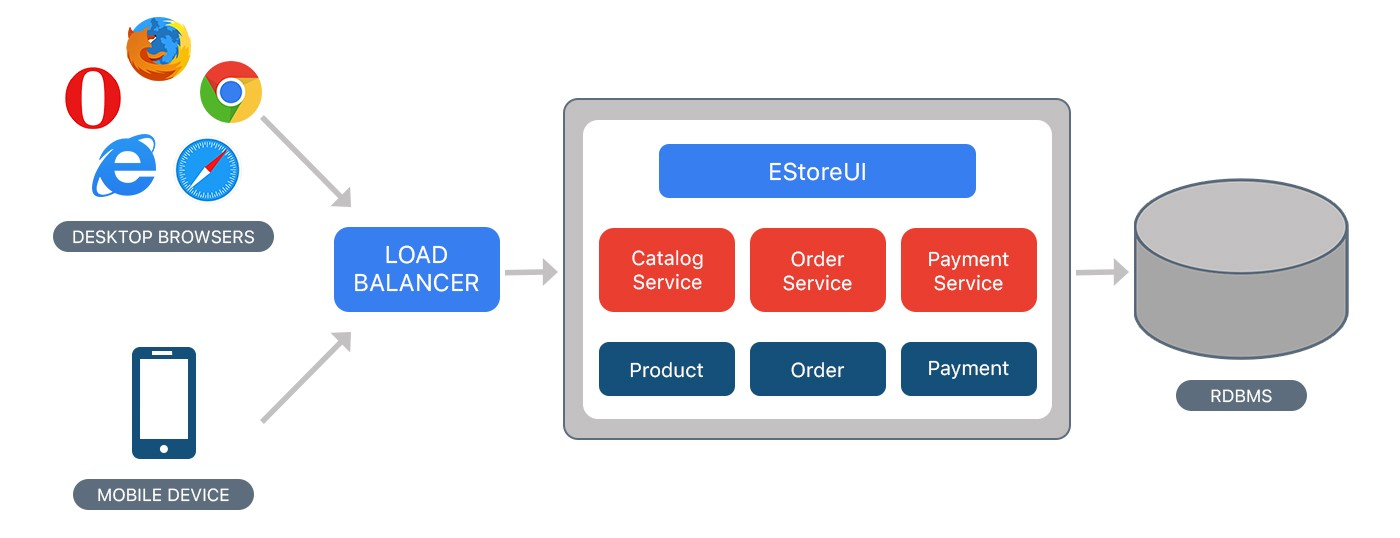
\includegraphics[keepaspectratio=true,scale=0.35]{img/monolith_arhichitecture.jpeg}
\caption{Arhitectura monolitic'a}
\label{monolith_arch}
\end{center}
\end{figure}
\textbf{Avantajele} arhitecturiii monolitice sunt: 
\begin{itemize}
\item[•]U'sor de dezvoltat - la 'inceputul unui proiect este mult mai u'sor s'a dezvol'ti o arhitectur'a monolitic'a.
\item[•]U'sor de testat. De exemplu, se pot implementa teste end-to-end prin simpla rularea a aplica'tiei 'si testarea ei cu un tool specializat.
\item[•]U'sor de pus 'in func'tiune, este necesar'a doar copierea pe un server 'si rularea programului.
\item[•]Scalabil'a pe orizontal'a prin rularea mai multor instan'te.
\end{itemize}
Arhitectura monolitic'a este abordarea tradi'tional'a care este folosit'a 'in multe sisteme, care sunt construite ca o aplica'tie autonom'a. Chiar dac'a este prezent'a 'in multe aplica'tii existente 'si 'inc'a este folosit'a pentru dezvoltarea aplica'tiilor noi, limit'arile 'si problemele existente 'in acest mod de abordare duc la cre'sterea popularit'a'tii arhitecturii bazate pe microservicii. \textbf{Dezavantajele} arhitecturii monolitice sunt:
\begin{itemize}
\item[•] Mentenan'ta - dac'a o aplica'tie este prea mare este foarte greu s'a faci schimb'ari rapide 'si s'a nu afectezi func'tionarea corect'a a altor componente.
\item[•]Dimensiunea aplica'tiei duce cre'sterea timpul de start-up.
\item[•]Toat'a aplica'tia va trebui restartat'a atunci c'and se face o schimbare de cod.
\item[•]Este foarte complicat de scalat.
\item[•]O problem'a 'in una dintree componente poate afecta 'intreaga aplica'tie.
\item[•]Este complicat s'a adopte tehnologii si framework-uri noi, deoarece prea multe lucruri trenuie schimbate 'in acela'si timp.
\item[•]Spre finalul ciclului de dezvoltare complexitatea de a scrie cod devine mai mare, iar raportul timp-eficien't'a devine tot mai mare.
\end{itemize}

Aceast'a arhitectur'a are 'si plusuri 'si minusuri, dar, dat fiind faptul c'a de fiecare dat'a c'and se rescrie o por'tiune de cod este necesar'a recompilarea 'intregului program, arhitectura monolitic'a  duce la 'intârzieri destul de mari, cauzate de compil'arile repetate a 'intregului program.

\section{Caracteristicile 'si avantajele arhitecturii orientate pe microservicii}
Microserviciile sunt ni'ste entit'a'ti mici, independente, autonome, create s'a func'tioneze 'impreun'a, fiecare dintre ele este focusat pe un singur lucru 'si  are scopul de a-l face bine.
Arhitectura bazat'a pe microservicii este un stil arhitectural care structureaz'a aplica'tia ca o colec'tie de servicii indepenedente 'si modulare, care sunt u'sor de testat, de 'intre'tinut 'si de 'in'teles.
Acest tip de abordare duce la cre'sterea agilit'a'tii prin 'imun'at'a'tirea productivit'a'tii 'si sc'aderea timpului de dezvoltare a produsului.
Microserviciile au demonstrat c'a sunt un sistem de nivel superior, 'in special pentru aplica'tii mari care sunt dezvoltate de mai multe echipe.
 Pe lâng'a beneficiile enumerate mai sus, microserviciile mai ofer'a urm'atoareele avantaje:
\begin{itemize}
\item[•] Sunt mentenabile.
\item[•] Sunt scalabile.
\item[•] Sunt u'sor de testat.
\item[•] Au nivel de cuplare joas'a.
\item[•] Sunt independente. 
\item[•] Sunt rezistente la c'aderi.
\item[•] Sunt organizate 'in func'tie de capabilit'a'tile 'si func'tionalit'a'tile de business.
\item[•] Ofer'a independen't'a dezvoltatorilor.
\item[•] Pot fi dezvoltate independent.
\item[•] Modific'arile pot fi aplicate u'sor, deoarece nu mai necesit'a recompilarea 'intregului produs.
\end{itemize}
\begin{figure}[H]
\begin{center}
\advance\leftskip-3cm
\advance\rightskip-3cm
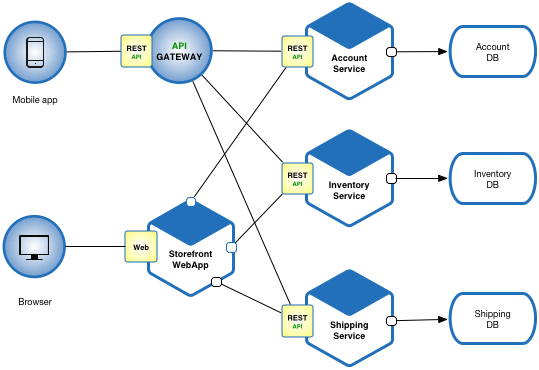
\includegraphics[keepaspectratio=true,scale=0.55]{img/Microservice_Architecture.png}
\caption{Arhitectura bazat'a pe microservicii}
\label{microservices_arch}
\end{center}
\end{figure}

Arhitectura bazat'a pe microservicii permite integrarea 'si livrarea continu'a a unui produs complex 'si de volum mare, deasemnea promoveaz'a diversitatea tehnologiilor utilizate 'intr-un proiect.
'In prezent, tot mai multe companii au 'inceput s'a foloseasc'a arhitecturi bazate pe microservicii pentru produsele lor. Câteva dintre aceste companii sunt\cite{microservice_companies}:
\begin{itemize}
\item[•] Netflix
\item[•] eBay
\item[•] Amazon
\item[•] Twitter
\item[•] PayPal
\item[•] SoundCloud
\item[•] Gilt
\item[•] The Guardian
\end{itemize}
Netflix, eBay 'si Amazon sunt cunoscute pentru arhitecturile lor diverse, care au evoluat de la \textit{Monolit} la \textit{Microservicii} cu scopul de a putea face fa't'a unor volume imense de date.

Totu'si, ca oricare alt'a solu'tie, arhitectura bazat'a pe microservicii are o serie de dezavantaje\cite{microservices_io}:
\begin{itemize}
\item[•] Se adaug'a complexitate din cauza cre'arii unor sisteme distribuite.
\item[•] Programatorul trebuie s'a implementeze comunicarea 'intre servicii.
\item[•] Testarea interac'tiunii este destul de complex'a.
\item[•] IDE-urile 'si tool-urile existente au un num'ar sc'azut de  func'tionalit'a'ti care ajut'a la dezvoltarea aplica'tiilor distribuite.
\item[•] Un sistem format din microservicii are un nivel mai ridicat al consumului de resurse.
\end{itemize}

\begin{figure}[H]
\begin{center}
\advance\leftskip-3cm
\advance\rightskip-3cm
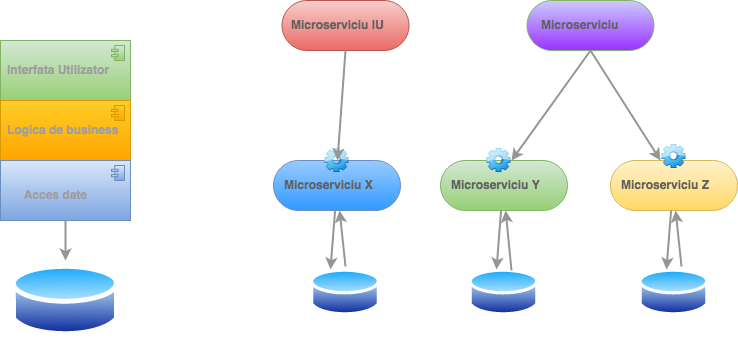
\includegraphics[keepaspectratio=true,scale=0.35]{img/microservices-vs-monolithic.png}
\caption{Diferen'ta dintre arhitecturi}
\label{microservices_vs_monolithic_arch}
\end{center}
\end{figure} 

Chiar dac'a mul'ti dezvoltatori sunt re'tinu'ti 'in vderea unei schimb'ari, sau ezit'a s'a 'incerce o abordare diferit'a, beneficiile microserviciilor sunt mult mai importante 'si mai semnificative decât dezavantajele, 'in cazul multor apliica'tii\cite{art_microservices}.
Arhitecturile modulare reduc riscul schimbarilor nedorite sau neanticipate dintr-o component'a 'in urma modific'arii altei componente. 'In concluzie, microserviciile sunt o parte misc'arii din industria IT care permite o colabor'are mai simpl'a 'intre echipe. Microserviciile nu sunt doar o tehnologie folosit'a 'in prezent, ele sunt un o cultur'a despre procesul de dezvoltare software.

\section{Microservicii 'in Cloud}

Resursele 'in \textit{Cloud} sunt disponiibile 'si puse la dispozi'tia atunci când sunt necesare. Comparativ cu o infrastructur'a clasic'a, nu exist'a o limit'a practic'a a acestora.
Diferite medii de dezvoltare 'si versiuni de servicii pot co-exista 'iin mod temporar sau permanent. Programatorul nu mai este nevoit s'a gheasc'a sau s'a calculeze cerin'tele 'si capacitatea de consum a sistemului. La cerere resursele pot fi scalate sau diminuate f'ar'a interven'tie 'in partea fizic'a a sistemului.

Faptul c'a pl'ate'sti doar ceea ce utilizezi reduce considerabil pre'tul experiment'arii, dar 'si cre'ste posibilit'a'tile de experimentare. Noi func'tiionalit'a'ti pot fi integrate, pot fi oprite 'si restartate cu noi parametri 'in cazul unui e'sec. Datorit'a cloudului se pot efectua numeroase experimente f'ar'a riscuri, acets lucru constituind cheia de succes a inova'tiei. Acest fapt se potrive'ste ideal cu conceptul de \textit{microservicii}, oferind posibilitatea de a atinge un nivel 'inalt de agilitate.

Programabilitatea cloud-ului permite automatizarea proceselor de dezvoltare 'si livrare.
Integrarea contnu'a este o parte a ciclului de via't'a a servicilor 'in cloud. Livrarea continu'a, pe de alt'a parte, introduce provoc'ri noi a complexit'a'ti de administrarea a multiplelor servicii 'in paralel.

Gândirea, perfec'tionarea continu'a, livrarea continu'a, managementul, monitorizarea 'si 'intre'tinerea API-urilor este o responsabilitate complex'a 'si consum'a extrem de mult timp. Sistemele Cloud ofer'a suport pentru acestea 'si u'sureaz'a via'ta dezvoltatorilor.

Arhitectura bazat'a pe microservicii este o abordare distribuit'a, dezvoltat'a pentru a rezolva limit'arile arhitecturii monolitice clasice. Microserviciile faciliteaz'a scalarea apliica'tiilor sau a anumitor module ale aplica'tiei. Totu'si sunt o provocare din punctul de vedere a complexit'a'tii arhitecturale 'si a oper'arii sistemului. Serviciile cloyd contribuie la reducerea acestei complexit'a'ti prin oferirea unor func'tionalit'a'ti preimplementate de management al serviciilor.

\section{Securitatea in sistemele informatice}


Securitatea aplica'tiilor cuprinde m'asurile luate pentru a asigura 'si a 'imbun'at'a'ti securitatea sistemului. Deseori aceasta este asigurat'a prin g'asirea, 'inl'aturarea 'si prevenirea vunlnerabilit'a'tilor de securitate. Sunt utiilizate mai multe tehnici pentru a ob'tine acest lucru, acestea pot fi aplicate la diferite etape ale ciclului de dezvolatare, cum ar fi: \textit{design, dezvoltare, livrare, perfec'tionare sau mentenan't'a}.

Sunt utilizate diferite abord'ari pentru a g'asi diferite subseturi ale vulnerabilit'a'tilor de securitate, acestea au un impact diferit prin cost, timp, efort 'si procentul de vulnerabiliit'a'ti ce pot fi detectate. Tehnicile esen'tiale sunt:
\begin{itemize}
\item \textit{Whitebox} - se refer'a la analiza securit'a'tii sau a codului. Aceast'a abordare poate fi adoptat'a doar de un inginer care 'in'telege deplin codul, 'si poate observa problemele prin analiza manual'a 'si vizual'a a codului surs'a.
\item \textit{Blackbox} - reprezint'a auditul 'in securitate. Opera'tia poate fi efectuat'a de un specialist 'in securitate, utilizând doar executabilul, f'ar'a necesitatea de analiza codul surs'a. Inginerul se concentreaz'a pe 'incerc'arile de a g'asi cazuri netratate care pot duce la compomiterea sistemului.
\item \textit{Revizuirea design-ului} - 'inainte de scrierea codului se analizeaz'a vulnerabilit'a'tile arhitecturale 'si ale dependen'telor externe ale sistemului.
\item \textit{Utilizarea tool-urilor} - 'in prezent exist'a un num'ar mare de tooluri automate care pot fi utilizate pentru detectarea problemelor de securitate, 'ins'a acestea au un num'ar mai mare de fals pozitive decât 'in cazurile de testare manual'a.
\item \textit{Platforme de vulnerabilit'a'ti coordonate} - sunt aplica'tii care ofer'a recompense hackerilor experimenta'ti pentru g'asirea de probleme de securitate.
\end{itemize}

Utilizarea acestor tehnici 'in mod adecvat 'imbun'at'a'te'ste calitatea sistemului prin 'inl'aturarea vulnerabilit'a'tilor. Acest proces este 'in totalitate responsabilitatea echipei de dezvoltare.

'In timp ce stocarea 'in sistemele cloud este convenabil'a 'si ofer'a posibilitatea de a accesa datele indiferent de loca'tie 'si or'a, de pe aproximativ orice dispozitiv cu conexiune la internet, securitatea sistemelor de sticare este o problem'a prioritar'a a organiza'tiilor IT 'si a departamentelor de securitate. Beneficiul principal al adopt'arii stoc'arii 'in cloud este asigurarea securit'a'tii si integriit'a'tii datelor cu caractez senzitiv.

Dezvoltatorilor sistemelor de cloud le apar'tine 'in totalitate responsabilitatea pentur securitatea aplica'tiilor lor. Ace'stia implementeaz'a 'in sistemele lor toate func'tionalit'a'tile esen'tiale pentru securitate, acestea fiind: \textit{autentificarea, autorizarea, controlul accesului 'si criptarea}. De aici 'in colo, fiecare companie are responsabilitatea de a ad'auga noi nivele de protec'tie pentru date 'si de a restric'tiona cât mai mult accesul la datele sensibile.

\subsection{Amenin't'ari}
Administratorii de sistem 'si dezvolatatorii de servicii software sunt mereu la straja securit'a'tii aplica'tiilor. 'Ins'a sunt numeroase probleme care par netriviale, 'ins'a pot compromite datele apliica'tiei. Principalele amenint'ari pentru securitatea aplica'tiilor sunt:
\begin{itemize}
\item \textit{Utilizatorii} - utilizatorii aplica'tiilor noastre sunt cea mai mare amenin'tare pentru propria lor integritate 'si pentru datele lor. Deseori ace'stia nu realizeaz'a cât de important e s'a accesezi doar partea sigur'a a internetului. Nerespectarea unor reguli de baz'a a navig'arii pe internet poate compromite parole, chei de acces, chei de criptare, orice efort din partea dezvoltatorilor de a p'astra securitatea va e'sua 'in acest caz.
\item \textit{Gre'seli elementare de structurare sau scriere a codului} - 'in ciuda multiplelor avertismente 'si a anilor de educa'tie 'inc'a exist'a cod cu gre'seli elementare de securitate. Problemele triviale sunt: \textit{SQL-injection} 'si\textit{Cross-site scripting}.O recomandare 'in acest'a direc'tie este utilizarea unor libr'arii specializate pentru SQL 'si pentru randare a datelor provenite de la utilizatori, acestea trateaz'a aceste cazuri 'si aplica'tia nu poate fi atacat'a 'in acest mod.

\item \textit{Utilizarea unor libr'arii 'invechite} - este recomandat s'a se utilizeze cele mai noi versiuni ale unor libr'arii 'si aplica'tii, aceste nu con'tin de obicei erorile 'si problemele de securitate cunoscute.
\item \textit{Setarea unor permisiuni de acces gre'site} - prin setarea permisiunilor de acces gre'site, utilizatorul poate ob'tine prea mult'a libertate 'si control asupra aplica'tiei. Este recomandat ca permisiunile s'a fie la nivelul minim necesar pentru utilizarea aplca'tiei conform modelului de cazuri de utilizare.
\item \textit{Hackerii} - persoanele care doresc s'a ob'tin'a profit sau date pre'tioase vor 'incerca mereu s'a strice aplica'tia, problema nu poate fi 'inl'aturat 'complet, dar procesul poate fi f'acut mai complex prin 'indeplinirea unor norme de securitate mai avansate.
\item \textit{Lipsa obfusc'arii sau cript'arii datelor} - datele stocate 'iin form'a citibil'a creaz'a o facilitate pentru hackerii, ace'stia nu mai au nevoie de munc'a suplimentar'a pentru ob'tinerea datelor valoroase odat'a ce au ob'tinut control asupra siistemului. 
\end{itemize} 
M'asurile esen'tiale pentru securitate vor fi discutate 'in sec'tiiunile ce urmeaz'a.
\subsection{Criptografia}
Criptografia - este utilizat'a pentru ascunderea mesajelor. Exist'a numeroase metode de criptare a datelor 'incepând cu Cifrul lui Caesar, una dintre cele mai primitive metode de criptare exiistente, terminând cu AES 'si RSA, acre sunt metodele de criptare standardizate, considerate aproape invincibile 'in momentul de fa't'a. Totu'si criptografia nu este o solu'tie general 'apentru securitate, aceasta este privit'a mai mult ca un \textit{tool}. Adversarul principal al criptografiei este - criptanaliza, 'stin'ta destinat'a descifr'arii mesajelor criptate prin analiza datelor de intrare 'si ie'sire ale unui algoritm.


\subsection{Compresia}

\subsection{Steganografia}

\section{Sisteme similare}
Acest capitol reprezint'a clasificarea si analiza sistemelor similare existente, bazat'a pe etapa de cercetare a proiectului. Sistemele au scop 'si functionalit'a'ti similare cu proiectul propus. Sistemele alese pentru compara'tie sunt:
\begin{itemize}
\item[•] CloudMe
\item[•] Dropbox
\item[•] CrashPlan
\item[•] ICloud
\item[•] Google Drive
\item[•] OneDrive
\item[•] pCloud
\item[•] sync.com
\end{itemize}
Dropbox, Google Drive, ICloud si OneDrive au fost incluse 'in acest studiu deoarece sunt 'in top 10 cele mai populare servicii de cloud 2019 \cite{topcloud}. Acestea reprezint'a un model pentru cum este v'azut un cloud storage modern: simplu de configurat, simplu de utilizat 'si disponibil la un pre't avantajos.
pCloud si sync.com sunt 'in topul sistemelor cu cea mai 'inalt'a recuritate de pe pia't'a. pCloud este categorizat ca un sistem infraudabil 'si nu a avut nici o expunere a datelor utilizatorilor. 'Ins'a aceste sisteme vin si cu pre'turi de 3-4 ori mai mari decât sistemele clasice.
\subsection{Metodologia de analiz'a}
'In ultimul deceniu tot mai mul'ti utilizatori, atât business cât 'si individuali, se baseaz'a pe stocarea fi'sierelor 'in Cloud.  Cele mai importante criterii pe care se bazeaz'a utilizatorii sunt: securitatea, simplitatea de utilizare a sistemului, disponibilitatea si pre'tul de utilizare. Analiza sistemelor individuale de cloud a fost efectuat'a 'in modul urm'ator:

Sunt sumarizate pre'turile de utilizare a sistemului 'si a diferitor op'tiuni. Sunt analizate detaliile capabilit'a'tilor tehnice 'si organiza'tionale ale p'ar'tii client 'si server a sistemului. Informa'tiile colectate sunt bazate pe sec'tiunile
{\it Terms of Service } 'si {\it Privacy Policy} ale documenta'tiilor oficiale ale sistemelor\cite{cloudstoragecomparison}.
Rezultatele analizei comparative au ca scop determinarea cerin'telor pricipale ale unui sistem de stocare cloud 'si compara'tia sistemului elaborat cu cele existente.
'In sec'tiunile ce urmeaz'a se vor analiza urm'atoarele func'tionalit'a'ti:

\begin{table}[H]
\caption{Criterii evaluare sisteme similare}
\small
\begin{tabular}{|c|c|c|c|c|c|c|c|}   
       
\hline                     
Copy & Backup & Sync & Sharing & \makecell{Client-side \\ Encryption} & \makecell{ Server-side \\ encryption} & Compression & Watermarking  \\ [0.1ex]   
%heading
\hline                              
\end{tabular}
  % titlul tabelului
\label{table:criteriatable}             
\end{table}

Pentru fiecare categorie din tabelul \ref{table:criteriatable} se va acorda un punctaj conform urm'atoarelor reguli:

\begin{itemize}
\item[\greencheck\greencheck] este echivalent pentru {\it foarte bine}, toate cerin'tele obligatorii pentru func'tionalitatea respectiv'a au fost 'indeplinite 'si câteva dintre cele op'tionale.
\item[\greencheck] este echivalent pentru {\it bine}, adic'a toate cerin'tele obligatorii pentru func'tionalitatea respectiv'a au fost 'indeplinite.
\item[\orangepm] este simbolul pentru {\it bine cu câteva vulnerabilit'a'ti}, nu toate cerin'tele esen'tiale au fost 'indeplinite.
\item[\redxmark] este echivalent cu {\it slab}, cel pu'tin o cerin't'a obligatorie nu a fost 'indeplinit'a.
\item[\redxmark \redxmark] este echivalentul pentru {\it foarte slab}, adic'a mai multe dintre cerin'tele obligatorii nu sunt indeplinite in func'tionalitatea respectiv'a sau func'tionalitatea lipse'ste.
\end{itemize}

\subsection{CloudMe}

\textbf{CloudMe}\cite{cloudme_com} este un sistem de cloud standard, care vine cu un serviciu de sincronizare 'si backup a fi'sierelor, dup'a o analiz'a detaliata ne putem da seama c'a acest sistem a fost inspirat din arhicunoscutul \textbf{Dropbox} care este analizat 'in sec'tiunea \ref{dropbox}. 

'In tabelul \ref{table:cloudmefeaturetable} sunt prezentate func'tionalit'a'tile sistemului 'si o not'a a fiec'arei func'tionalit'a'ti 'in concordan't'a cu evalu'arile primite pe pagina oficial'a a sistemului, precum 'si a vulnerabilit'a'tilor depistate 'in ultima perioad'a.

\begin{table}[H]
\centering
\small
\caption{CloudMe Func'tionalit'a'ti}
\begin{tabular}{|c|c|c|c|c|c|c|c|}          
\hline               
Copy & Backup & Sync & Sharing & \makecell{Client-side\\ Encryption} & \makecell{Server-side \\ encryption} & Compression & Watermarking \\ [0.5ex]   
%heading
\hline 
Da & Da & Da & Da & Da &  Nu & Nu & Nu    \\                      
\greencheck & \greencheck & \redxmark\redxmark & \orangepm & \greencheck\greencheck & \redxmark\redxmark &  \redxmark\redxmark &  \redxmark\redxmark  \\               
\hline                              
\end{tabular}
  % titlul tabelului
\label{table:cloudmefeaturetable}             
\end{table}

Tabelul \ref{table:cloudmesystemtable} prezint'a disponibilitatea \textbf{CloudMe} pe diferite platforme 'si pretul acestuia.
\begin{table}[H]
\centering
\caption{CloudMe Platforme disponibile 'si pre't}
\begin{tabular}{|c|c|c|c|}          
\hline                      
 Web Client & Desktop client & Mobile Client & 500GB Plan Price\\ [0.5ex]   
%heading
\hline                            
Da & Da & Da & 10\euro\\               
\hline                              
\end{tabular}
  % titlul tabelului
\label{table:cloudmesystemtable}             
\end{table}


Un fapt bun despre \textbf{CloudMe} este c'a acesta pune la dispozi'tia utilizatorului un spa'tiu de stocare gratuit de 3GB, iar pentru volume de date mai mari ofer'a op'tiuni la pre'tul mediu al pie'tei. Serviciul ofer'a func'tionalit'a'tile de baz'a, 'ins'a nimic desebit 'in materie de securitate. 

Interfa'ta web a \textbf{CloudMe} este foarte simpl'a si clar'a, este evident cum sa 'incarci un fisier sau cum sa 'il schimbi 'in alt folder.
\begin{figure}[H]
\begin{center}
\advance\leftskip-3cm
\advance\rightskip-3cm
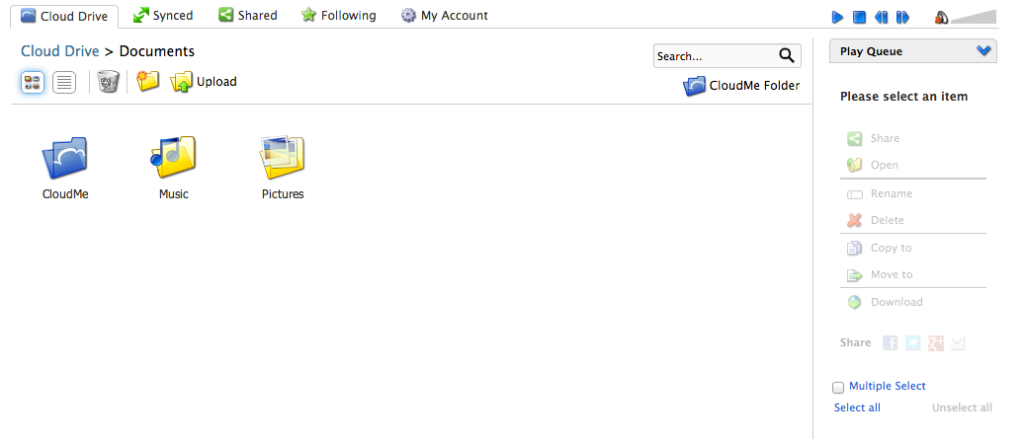
\includegraphics[keepaspectratio=true,scale=0.35]{img/Web-interface_CloudME.png}
\caption{CloudMe - interfa'ta web}
\label{web_cloudMe}
\end{center}
\end{figure}

\textbf{CloudMe} ofer'a sincronizarea aplica'tiilor pentru Windows, Mac, Linux, iOS 'si Android. Pentru ca sincronizarea sa poata avea loc utilizatorul prime'ste un a'sa numit "director albastru" ofer'a utilizatorului singronizare 'in timp real. De asemenea, \textbf{CloudMe} ofer'a op'tiunea de a alege timpul la care se va 'intâmpla sincronizarea.
Pentru a distribui fi'siere sunt disponibile mai multe op'tiuni, 'incepând cu distribuire clasic'a, care permite utilizatorului s'a ofere acces la fi'sierele lui prin distribuirea unui link, 'si ajungând la metode mult mai colaborative care permit altor utilizatori, c'arora li se ofer'a access, s'a modifice fi'sierele din cloud-ul altui utilizator sau s'a 'incarce fi'siere noi.

\begin{figure}[H]
\begin{center}
\advance\leftskip-3cm
\advance\rightskip-3cm
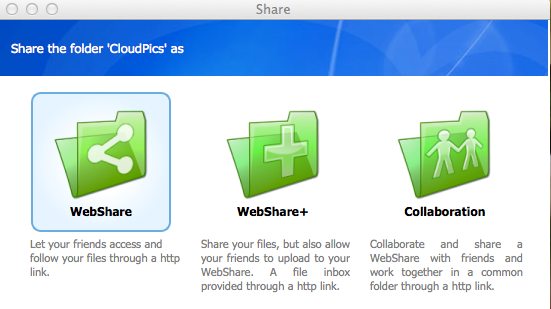
\includegraphics[keepaspectratio=true,scale=0.3]{img/Share-options_CloudME.png}
\caption{CloudMe - planuri de pre't}
\label{share_cloudMe}
\end{center}
\end{figure}

\textbf{CloudMe} arhiveaz'a  versiunile precedente ale fi'sierelor  prin func'tionalitatea co'sului de gunoi, care p'astreaz'a pentru 60 de zile toate fi'sierele care au fost 'sterse.

'In privin'ta securit'a'tii \textbf{CloudMe} nu este o op'tiune prea bun'a deoarece nu ofer'a criptarea datelor, acestea fiind vulnerabile pentru atacuri. Este posibil s'a 'incarci 'si s'a descarci fi'siere criptate, 'ins'a criptarea 'si decriptarea acestora ram'ane la latitudinea utilizatorului.


\textbf{CloudMe} este o aplica'tie foarte u'sor de utilizat 'si are o interfa't'a foarte intuitiv'a. Acesta dispune de func'tionalit'a'tile de baz'a ale unui sistem de stocare 'in cloud, 'ins'a nu este potrivit pentru stocarea fisierelor cu con'tinut de date senzitiv din cauza lipsei cript'arii, de asemnea atunci c'and fi'sierele sunt distribuite dup'a un link este foarte greu s'a determini cine a f'acut public un fi'sier cu caracter privat deoarece link-ul de acces poate fi u'sor furat.

Un alt defect al acestui sistem este func'tionalitatea de {\it Sync}, motivul pentru care i-am oferit punctaj minim este c'a 'in ultimul an a avut multiple vulnerabilit'a'ti, conform {\it CVE-2018-6892} \footnote{https://nvd.nist.gov/vuln/detail/CVE-2018-6892} atacatorii se puteau conecta la clientul de  "CloudMe Sync" prin portul 8888 'si trimiterea unor date mali'tioase puteau cauza "buffer overflow", acest lucru le oferea control asupra execu'tiei 'si posibilitatea de a executa cod mali'tios.


\subsection{Dropbox} \label{dropbox}


\textbf{Dropbox} a fost lansat in 2007 'si este definit ca unul dintre cele mai bune servicii de cloud pentru uz general\cite{cloudwards_best}. Sistemul are peste 500 de milioane de utilizatori 'in toat'a lumea, fiind unul dintre cele mai competitive servicii de pe pia't'a. 

'In tabelul \ref{table:dropboxfeaturetable} este prezentat'a o evaluare a sistemului pe baza unei evalu'ari personale, dar 'si pe baza evalu'arilor oferite de \textit{CloudWards}\cite{cloudwards_best} 'si \textit{On the Security of Cloud Storage Services}\cite{cloudstoragecomparison}.
\begin{table}[H]
\small
\centering
\caption{Dropbox Func'tionalit'a'ti}
\begin{tabular}{|c|c|c|c|c|c|c|c|}          
\hline               
Copy & Backup & Sync & Sharing & \makecell{Client-side\\ Encryption} & \makecell{Server-side \\ encryption} & Compression & Watermarking \\ [0.5ex]   
%heading
\hline 
Da & Da & Da & Da & Nu &  Da  & Nu & Nu    \\                      
\greencheck & \greencheck & \greencheck & \greencheck\greencheck & \redxmark\redxmark & \orangepm &  \redxmark\redxmark &  \redxmark\redxmark  \\               
\hline                              
\end{tabular}
  % titlul tabelului
\label{table:dropboxfeaturetable}             
\end{table}
'In tabelul \ref{table:dropboxsystemtable} sunt prezentate op'tiunile de clien'ti disponibili pentru \textbf{Dropbox} 'si oferta de pre't.
\begin{table}[H]
\centering
\caption{Dropbox Platforme disponibile 'si pre't}
\begin{tabular}{|c|c|c|c|}          
\hline                      
 Web Client & Desktop client & Mobile Client & 500GB Plan Price\\ [0.5ex]   
%heading
\hline                            
Da & Da & Da & 18\euro \\               
\hline                              
\end{tabular}
  % titlul tabelului
\label{table:dropboxsystemtable}             
\end{table}
\textbf{Dropbox} este u'sor de utilizat at'at utilizând aplica'tia web, cât 'si cea mobile sau desktop. 'In figura \ref{fig:web_Dropbox} este prezentat'a interfa'ta web a sistemului.

\begin{figure}[H]
\begin{center}
\advance\leftskip-3cm
\advance\rightskip-3cm
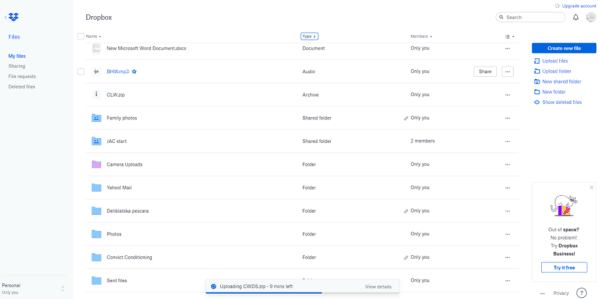
\includegraphics[keepaspectratio=true,scale=0.6]{img/dropbox-web-app.png}
\caption{Dropbox - interfa'ta web}
\label{fig:web_Dropbox}
\end{center}
\end{figure}

\textbf{Dropbox} ofer'a un serviciu de sincronizare "rapid 'si  inteligent", cu diverse posibilit'a'ti de customizare, 'ins'a aceast'a op'tiune poate fi aplicat'a doar pe anumite directoare, lucru care restrânge libertatea utilizatorului. 

Func'tionalitatea de partajare a fi'sierelor este ' in topul celor disponibile pe pia't'a deoarece ofer'a partajare atât de fi'siere cât 'si de directoare, cu parol'a sau f'ar'a, cu customizare de permisiune 'si termen de expirare. Se pot trimite link-uri pe mail sau prin copierea direct'a, link-urile pot fi 'sterse 'si fi'sierul nu mai este accesibil prin acel link. Aceast'a func'tionalitate este disponibil'a atât din orice aplica'tie \textbf{Dropbox}.

O func'tionalitate a c'arui autor este \textbf{Dropbox} este deduplicarea la nivel de bloc, prin 'imp'ar'tirea fi'sierului la 'inc'arcare 'in multiple por'tiuni de dimensiune fix'a 'si prin scanarea dac'a por'tiunea exist'a, acest lucru ofer'a o vitez'a de 'inc'arcare mai mare, dar prezint'a un risc deoarece un atacator poate  determina con'tinutul unui fi'sier de anumit format prin 'inc'arc'ari repetate de con'tinut diferit a anumitor por'tiuni, de exemplu un fi'sier cu analize medicale.

La nivel de securitate \textbf{Dropbox} nu este cea mai bun'a solu'tie, având un trecut destul de bogat 'in atacuri, suferind numeroase furturi de date. \textbf{Dropbox} salveaz'a fi'sierele 'in format criptat, 'ins'a numeroase metadate care includ 'si por'tiuni de text sunt salvate in format text. Acest lucru nu este benefic pentru utilizatori deoarece datele lor pot fi u'sor compromise. 


\textbf{Dropbox} a avut o evolu'tie specaculoas'a 'in ultimii 6  ani, adaugând numeroase noi func'tionalit'a'ti 'si devenind mult mai u'sor de utilizat. 'Ins'a \textbf{Dropbox} r'amâne o solu'tie pentru utilizatorii care nu au date senzitive stocate 'in acest sistem. Exist'a mai multe variante de compromitere a datelor, una dintre acestea este cauzat'a de implementarea FTS, prin pastrarea metadatelor pentru c'autare in format necriptat. Alta vulnerabilitate este cauzat'a de deduplicarea la nivel de bloc ce se execut'a la nivel de 'intreg sistem 'in loc de nivel fi'siere utilizator.

O vulnerabilitate de securitate a fost descoperit'a 'in 2018  {\it CVE-2018-12271}\footnote{https://www.cvedetails.com/cve/CVE-2018-12271/} atunci când un atacator se putea loga pe un cont \textbf{Dropbox} cu orice amprent'a arbitrar'a  'si avea access la toate fi'sierele  utilizatorului, un nivel suplimentar de securitate prin criptare cu cheie provenit'a de la utilizator ar fi prevenit acest lucru.


\subsection{CrashPlan}
\textbf{CrashPlan} este un sistem de stocare a fi'sierelor 'si backup care a ap'arut pe pia't'a 'in 2007. 'In prezent, sistemul a devenit unul foarte popular, zilnic acesta proceseaz'a peste 100 de miliarde de fi'siere. 

'In tabelul \ref{table:crashplanfeaturetable} sunt prezentate func'tionalit'a'tile sistemului 'si o evaluare efectiv'a a acestor capabilit'a'ti.
\begin{table}[H]
\small

\centering
\caption{CrashPlan Func'tionalit'a'ti}
\begin{tabular}{|c|c|c|c|c|c|c|c|}          
\hline               
Copy & Backup & Sync & Sharing & \makecell{Client-side\\ Encryption} & \makecell{Server-side \\ encryption} & Compression & Watermarking \\ [0.5ex]   
%heading
\hline 
Da & Da & Nu & Nu & Da &  Da  & Nu & Nu    \\                      
\greencheck & \greencheck & \redxmark\redxmark & \redxmark\redxmark & \greencheck\greencheck & \greencheck\greencheck &  \redxmark\redxmark &  \redxmark\redxmark  \\               
\hline                              
\end{tabular}
  % titlul tabelului
\label{table:crashplanfeaturetable}             
\end{table}
Din evaluarea de mai sus se observ'a c'a sistemul nu ofer'a partajare de fi'siere, 'in realitate aceast'a func'tionalitate a fost 'inl'aturat'a recent, cauza fiind riscul de compromitere a datelor. De asemenea partajarea fi'sierelor 'si men'tinerea unui nivel de securitate crescut implic'a un efort considerabil, de aceea, pentru moment, serviciul a fost deactivat.

'In tabelul \ref{table:crashplansystemtable} sunt prezentate platformele pe care este disponibil sistemul, se poate observa c'a pre'tul este mai mic comparabil cu adversarii analiza'ti 'in sec'tiunile precedente, acest fapt se poate datora lipsei unor anumite func'tionalit'a'ti.

\begin{table}[H]
\centering
\caption{CrashPlan Platforme  disponibile 'si pre'turi}
\begin{tabular}{|c|c|c|c|}          
\hline                      
 Web Client & Desktop client & Mobile Client & 500GB Plan Price\\ [0.5ex]   
%heading
\hline                            
Da & Da & No & 10\euro \\               
\hline                              
\end{tabular}
  % titlul tabelului
\label{table:crashplansystemtable}             
\end{table}

\textbf{CrashPlan} a fost caracterizat ca unul dintre cele mai bune sisteme pentru backup\cite{crashplan_review} datorit'a factorului c'a nu are dimensiune maxim'a a fi'sierelor pentru backup. Crashplan nu necesit'a implicare din partea utilizatorului pentru a executa copierea regulat'a a fi'sierelor. De asemenea, CrashPlan permite executarea opera'tiunii de backup 'in acela'si cont de utilizator a pân'a la 10 calculatoare.

 \textbf{CrashPlan} ofer'a mai multe nivele de securitate pentru fi'siere, toate datele sunt criptate de la client pân'a la server. Criptarea se execut'a utilizând o cheie de 448 bi'ti pentru utilizatorii unui plan pl'atit, pentru utilizatorii op'tiunii gratuite se utilizeaz'a o cheie de 128 bi'ti. Cheile de criptare sunt generate utiliz'and un sistem eficient de numere aliatoare.
De asemena exist'a op'tiunea de a selecta o cheie privat'a de criptare, acesta nu va fi salvat'a niciodata sub form'a de text 'si nu va fi accesibil'a nim'anui. 


Cel mai important lucru care face \textbf{CrashPlan} un sistem extrem de bun este performan'ta 'si eficien'ta cript'arii care ofer'a o securitate excep'tional'a a datelor, acestea nu pot fi decriptate f'ar'a cuno'stin'ta 'si acordul utilizatorului.
Datele utilizatorilor au fost compromise o singur'a dat'a, din cauza unui vulnerabilit'a'ti ce permitea executarea codului la distan't'a, acest lucru a devenit posibil  din cauza unei vulnerabilit'a'ti din clasa Java \textit{DateRMI}, descrierea vulnerabilit'a'tii poate fi g'asit'a 'in  {\it CVE-2017-9830} \footnote{https://www.cvedetails.com/cve/CVE-2017-9830/}.


\subsection{ICloud}
\textbf{ICloud} este unul dintre cele mai populare 'si utilizate sisteme de cloud conform CloudWards \cite{icloud_drive}, acest fapt nu este datorat doar pozi'tiei monopolistice pe care o ocup'a pe pia't'a, ci 'si func'tionalit'a'tilor pe care le ofer'a.

Sistemul \textbf{ICloud} este preinstalat pe toate dispozitivele Apple, acest lucru este deseori privit ca motivul pentru care este atât de popular. Totu'si, conform analizei func'tionalit'a'tilor, care este prezentat'a 'in tabelul \ref{table:icloudfeaturetable} se poate observa c'a func'tionalit'a'tile acestuia se ridic'a la un nivel destul de 'inalt.
\begin{table}[H]
\small
\centering
\caption{ICloud Func'tionalit'a'ti}
\begin{tabular}{|c|c|c|c|c|c|c|c|}          
\hline               
Copy & Backup & Sync & Sharing & \makecell{Client-side\\ Encryption} & \makecell{Server-side \\ encryption} & Compression & Watermarking \\ [0.5ex]   
%heading
\hline 
Da & Da & Da & Da & Da & Nu & Nu & Nu    \\                      
\greencheck & \greencheck & \greencheck\greencheck & \orangepm & \greencheck\greencheck & \redxmark\redxmark &  \redxmark\redxmark &  \redxmark\redxmark  \\               
\hline                              
\end{tabular}
  % titlul tabelului
\label{table:icloudfeaturetable}             
\end{table}
\begin{table}[H]
'In tabelul \ref{table:icloudsystemtable} sunt prezentate platformele pe care este disponibil \textbf{ICloud}.
\centering
\caption{ICloud Platforme disponibile 'si pre'turi}
\begin{tabular}{|c|c|c|c|}          
\hline                      
 Web Client & Desktop client & Mobile Client & 500GB Plan Price\\ [0.5ex]   
%heading
\hline                            
Da & Da & Da & 5\euro \\               
\hline                              
\end{tabular}
  % titlul tabelului
\label{table:icloudsystemtable}             
\end{table}

'Ins'a acesta are 'si câteva probleme  legate de clientul Desktop, care are func'tionalit'a'ti limitate, 'si limitarea func'tionalit'a'tii de partajare de fi'siere.\textbf{ICloud} ofer'a func'tionalitatea de sincronizare cu Apple Photos. Iar func'tionalitatea de share poate fi accesat'a din orice fi'sier care se afl'a 'intr-un director sincronizat.

'In 2014 a avut loc un furt de date de dimensiuni foarte mari, acesta a compromis reputa'tia ICloud, 'ins'a atacul a fost f'acut prin for't'a brut'a 'si "pescuirea datelor" de la viitoarele victime. 'In realitate apple ofer'a câteva func'tionalit'a'ti de securitate care 'il fac un sistem cu nivel de securitate peste media de pe pia't'a. 'Ins'a  Apple nu este un sistem cu "cuno'stin't'a zero", acesta stocheaz'a cheile de criptare 'in acela'si loc cu fi'sierele criptate, asta íl face extrem de vulnerabil 'in cazul unui atac.

Spre deosebire de alte sisteme, cum ar fi \textit{Google}\ref{google_drive}, este bine cunoscut c'a \textit{Apple} nu colaboreaz'a cu guvernul sau companiile publicitare 'si nu va oferi informa'tii private despre clien'tii s'ai.

\textbf{ICloud} nu este o solu'tie genral'a pentru stocarea fi'sierelor, acesta este potrivit pentru utilizatorii care nu au nevoie s'a p'astreze date extrem de sensibile din cauza posibilit'a'tii de decriptare prin brute force. Acesta nu este potrivit nici pentru utilizatorii care doresc o vitez'a ridicat'a de 'inc'arcare 'si dec'arcare a fi'sierelor, 'ins'a Apple continu'a s'a se perfec'tioneze 'si s'a creasc'a viteza opera'tiilor de re'tea.

De asemenea iCloud este extrem de vulnerabil pentru executare de cod la distan't'a conform datelor oferite de CVEDetails.com, vulnerabilit'a'tile recent descoperite sunt  {\it CVE-2018-20506}\footnote{https://www.cvedetails.com/cve/CVE-2018-20506/} 'si  {\it CVE-2018-4464}\footnote{https://www.cvedetails.com/cve/CVE-2018-4464/}, acest fapt este datorat popularit'a'tii sistemului crae 'il face o 'tint'a important'a pentru hackeri.



\subsection{Google Drive}\label{google_drive}
Cu aproximativ un miliard de utilizatori, \textbf{Google Drive} este cel mai popular serviciu de \textit{cloud} de pe pia't'a, aceast'a popularitate nu este datorat'a doar faptului c'a este preinstalat pe telefoanele Android, dar 'si capabilit'a'tilor de partajare 'si vitezei 'inalte de dec'arcare 'si 'inc'arcare a fi'sierelor. 

'In tabelul \ref{table:googledrivefeaturetable} sunt prezentate evalu'ari ale func'tionalit'a'tilor sistemului.
\begin{table}[H]
\small
\centering
\caption{Google Drive Func'tionalit'a'ti}
\begin{tabular}{|c|c|c|c|c|c|c|c|}          
\hline               
Copy & Backup & Sync & Sharing & \makecell{Client-side\\ Encryption} & \makecell{Server-side \\ encryption} & Compression & Watermarking \\ [0.5ex]   
%heading
\hline 
Da & Da & Da & Da & Da & Da & Da & Nu    \\                      
\greencheck & \greencheck\greencheck & \greencheck & \greencheck & \greencheck\greencheck & \greencheck &  \orangepm &  \redxmark\redxmark  \\               
\hline                              
\end{tabular}
  % titlul tabelului
\label{table:googledrivefeaturetable}      
\end{table}

De'si \textbf{Google Drive} ofer'a criptarea datelor, securitatea si intimitatea nu sunt punctele forte ale sistemului, acesta având antecedente de implicare 'in campaniile miltare de colectare a datelor 'si spion'arii cet'a'tenilor.  Compresia datelor, pe de alt'a parte, se refer'a la reducerea dimensiunii imaginilor, proces de compresie cu pierderi.

'In tabelul \ref{table:googledrivesystemtable} sunt prezentate op'tiunile de client disponibile pentru \textbf{Google Drive}, de asemenea fiecare utilizator prime'ste ini'tial 10 GB de stocare gratuit'a.
\begin{table}[H]
\centering
\caption{Google Drive Platforme Disponibile 'si Pre'turi}
\begin{tabular}{|c|c|c|c|}          
\hline                      
 Web Client & Desktop client & Mobile Client & 500GB Plan Price\\ [0.5ex]   
%heading
\hline                            
Da & Da & Da & 15\euro \\               
\hline                              
\end{tabular}
  % titlul tabelului
\label{table:googledrivesystemtable}             
\end{table}

Google Drive este unul dintre cele mai bune sisteme pentru colaborare, ocupând locul 2, dup'a Dropbox, prezentat 'in sec'tiunea \ref{dropbox}. Punctul forte al colabor'arii oferite de Google Cloud este faptul c'a Office Suite este integrat 'in acest sistem. 

Func'tionalitatea de sincronizare este extrem de performant'a, dar nu ofer'a sincronizare la nivel de bloc de fisier. Partajarea de fi'siere este una dintre cele mai folosite func'tionalit'a'ti ale sistemului, 'ins'a acesta vine cu câteva vulnerabilit'a'ti cauzate de lipsa cript'arii la partajare sau protejarea cu parol'a. Partajarea este u'sor de executat link-ul poate fi partajat prin email, Facebook, Twitter sau copiat 'si salvat 'in destina'tia dorit'a.

Datele sunt criptate utilizând AES-128 atunci când sunt salvate pe disc 'si prin TSL atunci când sunt transportate 'intre client 'si server. Oricum sistemul nu ofer'a "zero-knowledge" 'si oricine de'tine are control asupra sistemului poate s'a citeasc'a datele ( exemplu: programatorii sistemului).  
Totu'si pentru o protec'tie mai bun'a Google ofer'a posibilitatea de autentificare 'in 2 pa'si.


Google Drive vine cu foarte multe aplica'tii integrate 'si posibilt'a'ti de colaborare integrate 'in sistem. Autentificare 'in 2 pa'si, criptare a datelor  'si vitez'a ridicat'a de 'inc'arcare 'si desc'arcare, dar lipsa posibilit'a'tii de criptare privat'a 'si vulnerabilit'a'tile cauzate de lipsa unei cript'ari destul de sigure pentru func'tionalitatea de partajare de fi'siere fac \textbf{Google Cloud} sa nu fie cea mai bun'a solu'tie pentru securitatea 'si integritatea datelor.

\subsection{OneDrive}
 
\textbf{OneDrive} este un sistem de stocare 'in cloud dezvoltat de compania MIcrosoft, are un trecut destul de ambiguu 'in privin'ta securit'a'tii datelor, de'si 'si-a perfec'tionat securitatea, nu poate fi 'incadrat 'in topul celor mai sigure sisteme de securitatea\cite{top_secure}, 'ins'a tinde spre acesta.

Analiza func'tionalit'a'tilor sistemului este prezentat'a 'in tabelul \ref{table:onedrivefeaturetable}.
\begin{table}[H]
\small

\centering
\caption{OneDrive Func'tionalit'a'ti}
\begin{tabular}{|c|c|c|c|c|c|c|c|}          
\hline               
Copy & Backup & Sync & Sharing & \makecell{Client-side\\ Encryption} & \makecell{Server-side \\ encryption} & Compression & Watermarking \\ [0.5ex]   
%heading
\hline 
Da & Da & Da & Da & Nu & Da & Nu & Nu    \\                      
\greencheck & \greencheck\greencheck & \greencheck & \greencheck & \redxmark\redxmark & \redxmark\redxmark &  \redxmark\redxmark &  \redxmark\redxmark  \\               
\hline                              
\end{tabular}
  % titlul tabelului
\label{table:onedrivefeaturetable}             
\end{table}
Func'tionalit'a'tile nu au primit o not'a maxim'a din cauza ambiguit'a'tii de utilizare a sistemului, 'in dependen't'a de tipul fi'sierului selectat, meniurile arat'a diferit, uneori poate fi o problem'a pentru utilizatori. De asemenea, sistemul nu este unul cu cuno'stin'te zero, atacatorul poate ob'tine datele unui utilizator, odat'a ce s-a infiltrat 'in sistem, deoarele toate datele necesare pentru decriptare sunt deja prezente 'in sistem.

'In tabelul \ref{table:onedrivesystemtable} sunt prezentate datele cu privire la disponibilitatea sistemului pe diferite platforme, dar 'si pre'tul unui abonament cu spa'tiu de stocare de 500GB.
\begin{table}[H]
\centering
\caption{OneDrive Platforme Disponibile 'si Pre'turi}
\begin{tabular}{|c|c|c|c|}          
\hline                      
 Web Client & Desktop client & Mobile Client & 500GB Plan Price\\ [0.5ex]   
%heading
\hline                            
Da & Da & Da & 15\euro \\               
\hline                              
\end{tabular}
  % titlul tabelului
\label{table:onedrivesystemtable}             
\end{table}
\textbf{OneDrive} urmeaz'a ni'ste principii definite de Dropbox cu privire la standardele de sincronizare a fi'sierelor. OneDrive obi'snuia s'a aib'a probleme serioase cu privire la securitate, neavând nici criptare la nivelul nivelului de stocare. 'In prezent, âns'a sistemul ofer'a criptare la transmitere 'si la stocare. Criptarea nivelului de stocare include 2 componente esen'tiale: \textit{BitLocker}, criptare la nivel de disc, 'si un sistem de criptare per fi'sier a con'tinutului.
Fiecare fi'sier este securizat priin utilizarea unei chei AES unice de 256 de biti, de asemenea se folose'ste protocolul TLS pentru a preveni atacurile de tipul \textit{man-in-the-midle}
Dar minusul acestui sistem este c'a cheile sunt stocate pe acela'si sistem, orice angajat poate eventual s'a citeasc'a datele utilizatorilor sau s'a le ofere companiilor de e-publicitate sau unor servicii secrete.

'In concluzie, \textbf{OneDrive} este un sistem care a evoluat considerabil 'in ultima perioad'a, 'ins'a are neajunsuri considerabile pe partea de securitate. De asemenea sistemul nu ofer'a func'tionalitate de comopresie, ceea ce cre'ste costulm de stocare a datelor, datele pot fi compresate de utilizator 'in prealabil, iar dup'a desc'arcare acestea pot fi decompresate, opera'tia 'ins'a este anevoioas'a 'si prezint'a o problem'a 'in cazul partaj'arii fi'sierelor. Sistemul nu este potrivit pentru stocarea unor date sensibile 'si este recomandat doar pentru stocarea unor date netriviale.


\subsection{pCloud}

pCloud a fost fondat 'in 2013 'si 'in doar 3 ani a ajuns la peste 3 milioane de utilizatori,  competitorii cei mai importan'ti sunt  Dropbox 'si Copy. Chiar dac'a este nou pe pia't'a, spre deosebire de competitorii s'ai mari, acesta ofer'a func'tionalit'a'ti de top 'si este inclus 'in topul \textit{Most Secure Cloud Storage 2019: Safety First}\cite{top_secure}.

pCloud ofer'a func'tionalit'a'tile de sincronizare, backup (se opoate aplica 'si pe datele de pe Instagram sau Facebook), colaborare 'si criptare avansat'a a datelor. O evaluare a acestor capabilit'a'ti este oferit'a 'in tabelul \ref{table:pcloudfeaturetable}.

\begin{table}[H]
\centering
\caption{Func'tionalit'a'ti}
\begin{tabular}{|c|c|c|c|c|c|c|c|}          
\hline               
Copy & Backup & Sync & Sharing & \makecell{Client-side\\Encryption} & \makecell{Server-side\\encryption} & Compression & Watermarking \\ [0.4ex]   
%heading
\hline 
Da & Nu & Da & Da & Da & Da & Nu & Nu    \\                      
\greencheck & \redxmark\redxmark & \greencheck & \greencheck & \greencheck\greencheck & \greencheck\greencheck &  \redxmark\redxmark &  \redxmark\redxmark  \\               
\hline                              
\end{tabular}
  % titlul tabelului
\label{table:pcloudfeaturetable}             
\end{table}
Sistemul este prezent pe toate tipurile de platforme, tabelul \ref{table:pcloudsystemtable} 'si are un pre't  destul de ridicat, 'ins'a rezonabil pentru un sistem securizat de stocare.
\begin{table}[H]
\centering
\caption{Sisteme de operare}
\begin{tabular}{|c|c|c|c|}          
\hline                      
 Web Client & Desktop client & Mobile Client & 500GB Plan Price\\ [0.5ex]   
%heading
\hline                            
Da & Da & Da & 40\euro \\               
\hline                              
\end{tabular}
  % titlul tabelului
\label{table:pcloudsystemtable}             
\end{table}

Securitatea este unul dintre punctele forte ale sistemului, dezvoltatorii 'incearc'a s'a ofere servicii la cel mai 'inalt nivel 'si sa ofere func'tionalit'a'ti care nu sunt prezente la competitori. Sistemul folose'ste key de 256 biti 'si TSL pentru transmisia de date. Securitatea 'ins'a vine 'si cu un pre't, fi'sierele nu pot fi modificate 'in sistem, deoarece opera'tiile de criptare 'si decriptare ar trebui efectuate repetat, provocând costuri de prelucrare ridicate. De asemenea, sediul central al companiei se afl'a 'in Elve'tia, unde sunt cele mai stricte reguli de protec'tie a datelor, astfel utilizatorul poate fi lini'stit cu privire la integritatea datelor sale.

Datele 'inc'arcate sunt repartizate 'in func'tie de tipul de date: imagini, documente, muzica 'si video.

Un dezavantaj al sistemului este c'a criptarea este o func'tionalitate care nu este oferit'a 'in pachetul de baz'a 'si are un pre't mai ridicat, comparativ cu  alte sisteme care ofer'a criptarea ca serviciu gratuit.



\subsection{sync.com}
\textbf{Sync.com} a fost fondat 'in 2011 de c'atre Suhan Shan, Thoman Savundra, 'si Darius Antia. Acesta a devenit deja un competitor serrios pentru Google Drive si Dropbox. Caracteristicile pentru care a ajuns atât de popular sunt analizate 'in tabelul \ref{table:syncfeaturetable}.

\begin{table}[H]
\small
\centering
\caption{Func'tionalit'a'ti}
\begin{tabular}{|c|c|c|c|c|c|c|c|}          
\hline               
Copy & Backup & Sync & Sharing & \makecell{Client-side\\ Encryption} & \makecell{Server-side \\ encryption} & Compression & Watermarking \\ [0.5ex]   
%heading
\hline 
Da & Da & Da & Da & Da & Da & Nu & Nu    \\                      
\greencheck & \greencheck\greencheck & \greencheck & \greencheck & \greencheck\greencheck & \greencheck\greencheck &  \redxmark\redxmark &  \redxmark\redxmark  \\               
\hline                              
\end{tabular}
  % titlul tabelului
\label{table:syncfeaturetable}             
\end{table}
Din p'acate sistemul nu ofer'a compresia sau deduplicarea datelor, sistemul stocând volumul real de date pe care 'il prime'ste de la utilizator, plus câteva metadate create de algoritmii de compresie.
\begin{table}[H]
\centering
\caption{Sisteme de operare}
\begin{tabular}{|c|c|c|c|}          
\hline                      
 Web Client & Desktop client & Mobile Client & 500GB Plan Price\\ [0.5ex]   
%heading
\hline                            
Da & Da & Da & 15\euro \\               
\hline                              
\end{tabular}
  % titlul tabelului
\label{table:syncsystemtable}             
\end{table}
Criptarea datelor face ca sistemul s'a nu mai poat'a interpreta datele stocate, astfel sistemul nu ofer'a posibilitatea de deschidere 'si vizualizare a fi'sierelor, doar dec'arcarea 'si manipularea lor ulterioar'a cu alte aplica'tii. 'Ins'a exist'a 'si op'tiunea de a stoca fi'sierele f'ar'a criptare. Caracteristicile cheie ale sync.com sunt :
\begin{itemize}
\item[•] {Cunostin'te zero despre date}
\item[•] {Criptare privat'a}
\item[•] {U'sor de utilizat}
\item[•] {Syncronizare}
\item[•] {Partajare de fi'siere cu control asupra opera'tiei}
\end{itemize}

\textbf{Sync} este unul dintre sistemele care garanteaz'a securitate la nivelul cel mai 'inalt, acest sistem folose'ste pentru criptare RSA cu chei 'intre 512 si 2048 biti. Sync nu p'astreaz'a cheile de criptare 'in sistem, daca utilizatorul 'i'si uit'a parola atunci datele lui nu vor putea fi recuperate niciodat'a. De asemenea se poate activa 'si op'tiunea de autentificare 'in doi pa'si, pentru a oferi o protec'tie 'si mai bun'a.

Sistemul ofer'a func'tionalitatea de sincronizare, 'ins'a nu orice director poate fi selectat pentru efectuarea opera'tieidin cauza faptului c'a se iau 'in considerare particularit'a'tile fiec'arei aplicatii. 
Sync ofera func'tionalitatea de partajare de fi'siere care poate fi configurat'a ad'augând parol'a sau timp de expirare.


Nu putem nega c'a sync.com ofer'a o func'tionalitate de criptare complex'a 'si eficient'a care ofer'a o securitate avansat'a, dar, partea negativ'a a acestui lucru este c'a atunci c'and dorim s'a vizualiz'am un fi'sier sau s'a'il desc'arc'am, opera'tia ar putea dura 'intre c'ateva secunde 'si cateva minute din cauza complexit'a'tii ad'augate de criptare.


\subsection{Concluzii 'si plasarea sistemului}
Volumul de date stocate 'in cloud a crescut cu un factor de 40 'in ultimii 10 ani, cre'sterea este constant'a.  Evolu'tia tehnologic'a aduce un pre't mai mic pentru componentele hardware de stocare, dar 'si cantit'a'ti mai mari de date ceea ce 'impiedic'a sc'aderea pre'tului serviciilor. De asemnea, evolu'tia tehnologic'a aduce un impact negativ 'si asupra securit'a'tii, un atac de for't'a brut'a poate fi executat mult mai u'sor pe un sistem mai performant.

Dup'a studiul efectuat, am determinat c'a nici un sistem nu ofer'a functionalitatea de compresie de fi'siere, cu toate c'a unele sisteme ofer'a deduplicare, aceasta vine cu un impact asupra securit'a'tii utilizatorilor. Sistemul propus ofer'a reducerea volumului de date prin algoritmi de compresie 'si decompresie f'ar'a pierderi, spre deosebire de Google care efectueaz'a compresia imaginilor 'in versiunea gratuit'a prin reducerea dimensiunii, se pierde calitatea imaginii 'si este o experient'a nepl'acut'a pentru utilizatori. Analiza comparativ'a este prezentat'a 'in tabelul \ref{table:comparationtable}.


\begin{table}[H]
\small
\centering
\caption{Compara'tie sisteme similare}
\begin{tabular}{|c|c|c|c|c|c|c|c|}          
\hline               
Nume & Copiere & Partajare & \makecell{Criptare\\ la \\partajare }& \makecell{Criptare\\ pe disc} & \makecell{Algoritmi \\adaptivi} & Compresie & \makecell{Stegano-\\grafie} \\ [0.5ex]   
%heading
\hline 
CloudMe & \greencheck & \greencheck & \greencheck & \redxmark & \redxmark & \redxmark & \redxmark \\    
\hline           
Dropbox & \greencheck & \greencheck & \redxmark & \greencheck & \redxmark & \greencheck & \redxmark \\               
\hline
CrashPlan & \greencheck & \redxmark & \redxmark & \greencheck & \redxmark & \redxmark & \redxmark \\   
\hline
ICloud & \greencheck & \greencheck & \redxmark & \greencheck & \redxmark & \redxmark & \redxmark \\   
\hline
GDrive & \greencheck & \greencheck & \redxmark & \greencheck & \redxmark & \greencheck & \redxmark \\   
\hline
OneDrive & \greencheck & \greencheck & \redxmark & \redxmark & \redxmark & \redxmark & \redxmark \\   
\hline
pCloud & \greencheck & \greencheck & \greencheck & \greencheck & \redxmark & \redxmark & \redxmark \\   
\hline
sync.com & \greencheck & \greencheck & \greencheck & \greencheck & \redxmark & \redxmark & \redxmark \\   
\hline
\textcolor{red} {Bitstored} & \greencheck & \greencheck & \greencheck & \greencheck & \greencheck & \greencheck & \greencheck \\               
\hline                              
\end{tabular}
  % titlul tabelului
\label{table:comparationtable}             
\end{table}
Majoritatea sistemelor ofer'a criptarea datelor, unele au metode imposibil de spart, altele au metode mai simple 'si pu'tin sigure. Sistemul propus cripteaz'a datele utilizatorului utilizând algoritmi auto-calibrabili  care evolueaz'a 'in func'tie de sistemul pe care ruleaza aplica'tia sau de trecerea timpului. De asemenea sistemul folose'ste cei mai noi si siguri algoritmi TwoFish 'si PBFK2, care au fost modifica'ti s'a foloseasc'a key mai sigure de o lungime de 256 'si 512 bi'ti.

Un aport nou pe care 'il aduce sistemul 'si nu a fost observat la niciuna dintre aplica'tiile studiate este semn'atura pe fi'siere, pentru a detecta furtul de date prin extragerea codului - tehnica folosit'a este steganografia.


	Sistemul elaborat este mai mult un prototip, care poate fi dezvoltat, devenind un competitor pentru cele enumerate mai sus. Se pot ad'auga func'tionalit'a'ti suplimentare pe partea de partajare de fi'siere. 


\chapter{Analiz'a 'si Fundamentare Teoretic'a}
\label{ch:analysis}

\section{Cazuri de utilizare}
\begin{figure}[H]
\begin{center}
\advance\leftskip-3cm
\advance\rightskip-3cm
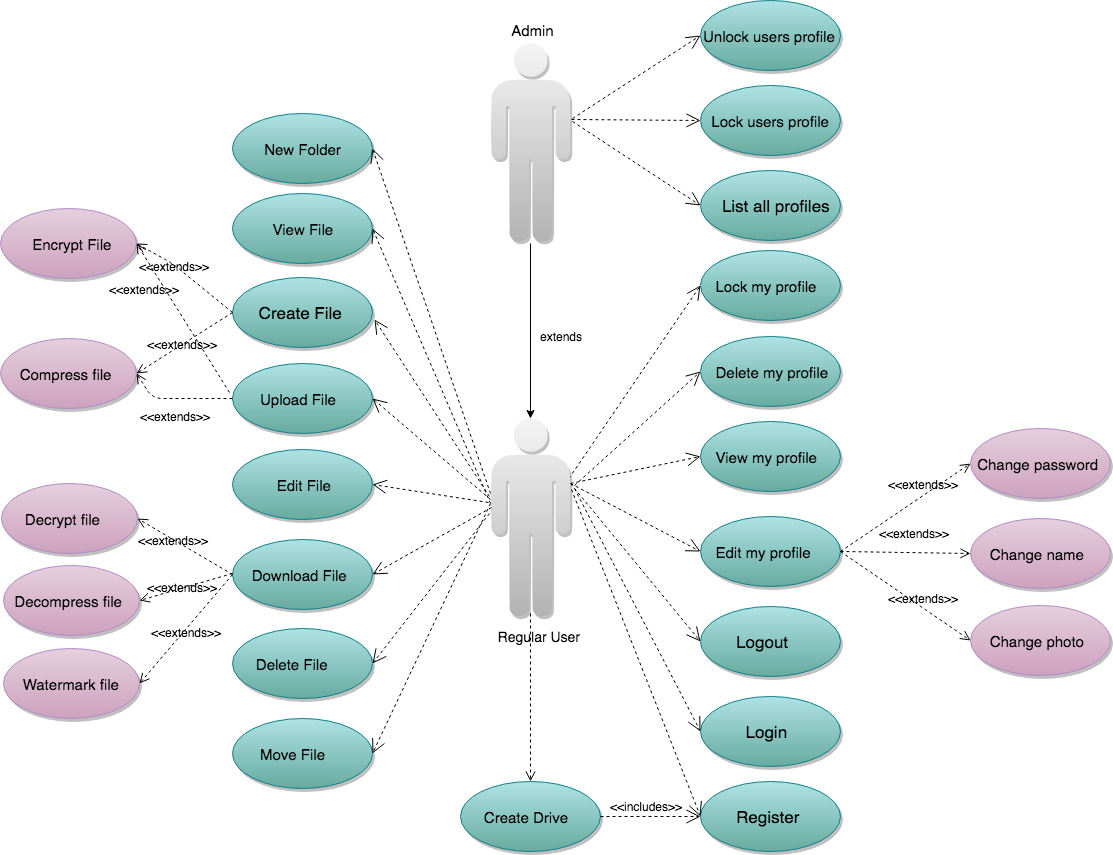
\includegraphics[keepaspectratio=true,scale=0.4]{img/use_case_diagram.png}
\caption{Use cases}
\label{use_cases_diagram}
\end{center}
\end{figure}
\subsection{Actori}
\subsection{Modele de cazuri de utilizare}
\section{Arhitectura canceptual'a a sistemului}

\section{Tehnologii}
\subsection{Golang}
Golang  este un limbaj de programare care a ap'arut 'in 2007. Este un limbaj care care ofera analiz'a static'a a codului: \textit{gofmt} - formatarea static'a a codului, \textit{golint} - stilizarea codului, \textit{godoc} - documentarae codului, acestea ofer'a o siguran't'a asupra codului scris. 'In figura \ref{golang_pic} este reprezentat'a emblema oficial'a a Golangului.
\begin{figure}[H]
\begin{center}
\advance\leftskip-3cm
\advance\rightskip-3cm

\includegraphics[keepaspectratio=true,scale=0.15]{img/golang.png}
\caption{Golang}
\label{golang_pic}
\end{center}
\end{figure}

Go ofer'a un tool pentru testare integrat 'in limbaj, acesta a fost elaborat pentru simplitate 'si oficien't'a. Golang ofer'a un API foarte simplu care poate fi folosit pentru orice tip de teste.



\subsection{gRPC}
\subsection{VueJS}
\subsection{MongoDB}
\subsection{Couchbase}
\subsection{HTML, CSS, Bootstrap}
\subsection{JSON Web Token(JWT)}
\subsection{Docker 'si Kubernetes}
\subsection{Google Cloud}
\subsection{Git}

\chapter{Proiectare de Detaliu 'si Implementare}
Acest capitol prezint'a deciziile 'si pa'sii de implementare parcur'si 'in ciclul de dezvoltare al proiectului. Sistemul propus este format din 3 subsisteme: aplica'tia web; serverul, care este format din alte subsisteme, 'si bazele de date. Capitolul va oferi o descriere succint'a a tuturor componentelor, incluzând 'sabloanele arhitecturale, 'sabloanele de design 'si algoritmii folositi 'in dezvoltarea proiectului.
\section{Arhitectura serverului}
\subsection{Descriere general'a}
Pentru dezvoltarea aplica'tiei de server, principala tehnologie folosit'a a fost Golang, pentru unul dintre module s-a folosit Python.
Pentru structura proiectului am ales 'sablonul arhitectural bazat pe microservicii, 'sablonul 'si avantajele au fost descrise 'in sec'tiunea 3.2.
Secviciile din care este compus serverul sunt:
\begin{enumerate}
\item Authentication service (descris 'in \ref{s_auth})
\item Compression service  (descris 'in \ref{s_compession})
\item Crypto service  (descris 'in \ref{s_crypto})
\item File service  (descris 'in \ref{s_file})
\item Logging service  (descris 'in \ref{s_logging})
\item Watermarking service  (descris 'in \ref{s_watermarking})
\item User service  (descris 'in \ref{s_user})
\end{enumerate}
Arhitectura sistemului este prezentat'a 'in figura \ref{system_architecture}
\begin{figure}[H]
\begin{center}
\advance\leftskip-3cm
\advance\rightskip-3cm
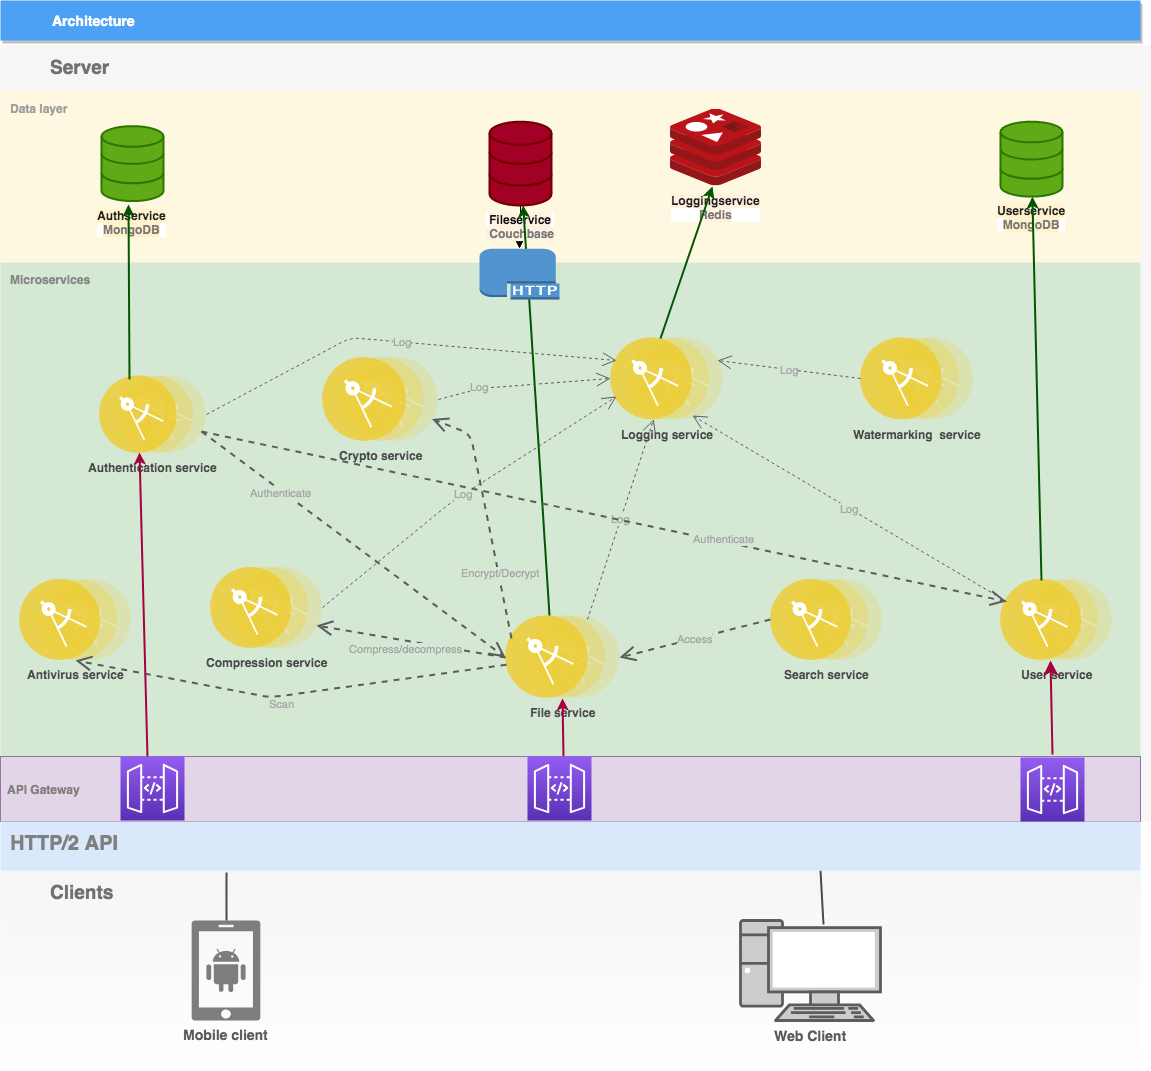
\includegraphics[keepaspectratio=true,scale=0.43]{img/diagrama_sistem.png}
\caption{Arhitectura sistemului}
\label{system_architecture}
\end{center}
\end{figure}
De asemenea pentru dezvoltarea serverului au fost folosite 2 tipuri de baze de date: MongoDB 'si Couchbase. Ambele fiind accesibile doar prin serverul dedicat. Pentru orchestrarea 'si punerea 'in func'tiune a microserviciilor am folosit Docker si kubernetes. Pentru maparea API-urilor am folosit evnvoy 'si Docker.
\subsection{Orchestrarea microserviciilor}
 Microserviciile sunt o modalitate de a desp'ar'ti func'tionalit'a'tile dintr-un sistem. Acestea ne ofer'a flexibilitatea de a scala func'tionalit'a'ti specifice 'si de a fi agili 'in livrarea produselor.
Dup'a ce func'tionalit'a'tile au fost separate 'in subsisteme dedicate, 'intrebarea urm'atoare ar fi: cum s'a le "lipim" la loc?

'In procesul de stabilire a comunic'arii 'intre servicii am avut o provocare destul de mare: s'a p'astrez cuplarea la un nivel cât mai jos, 'in caz contrar ar putea ap'area: multiple c'aderi, testare necalitattiv'a, dificultate crescut'a de 'in'telegere 'si costuri crescute de consum.




\subsection{Microserviciul de autentificare}  \label{s_auth}
\subsubsection{Introducere}
\subsubsection{Arhitectur'a}

\begin{figure}[H]
\begin{center}
\advance\leftskip-3cm
\advance\rightskip-3cm
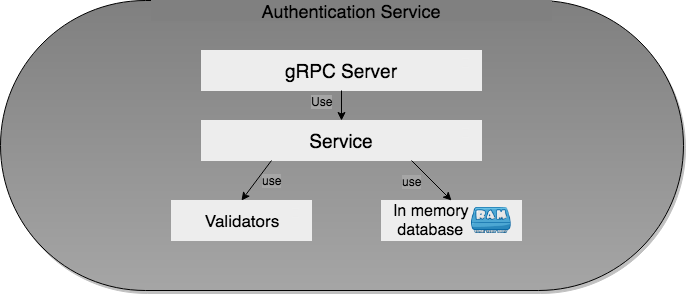
\includegraphics[keepaspectratio=true,scale=0.4]{img/auth_arch.png}
\caption{Arhitectura serviciului de autentificare}
\label{auth_arch}
\end{center}
\end{figure}

\subsubsection{Rezultate ob'tinute}


\subsection{Microserviciul de criptare} \label{s_crypto}
\subsubsection{Introducere}
\subsubsection{Arhitectur'a}

\begin{figure}[H]
\begin{center}
\advance\leftskip-3cm
\advance\rightskip-3cm
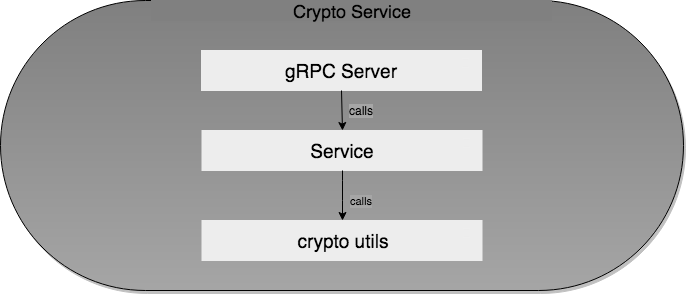
\includegraphics[keepaspectratio=true,scale=0.4]{img/crypto_arch.png}
\caption{Arhitectura serviciului de criptare}
\label{crypto_arch}
\end{center}
\end{figure}

\subsubsection{Rezultate ob'tinute}


\subsection{Microserviciul de steganografie 'si marcare}  \label{s_watermarking}

\subsubsection{Introducere}
Steganografia este 'stiin'ta ascunderii mesajelor, numele provenind de la cuvintele grese'sti \textit{steganos'}, care 'inseamn'a protejat, ascuns, 'si \textit{graphein}, care 'inseamn'a a scrie.
\subsubsection{Arhitectur'a}

\begin{figure}[H]
\begin{center}
\advance\leftskip-3cm
\advance\rightskip-3cm
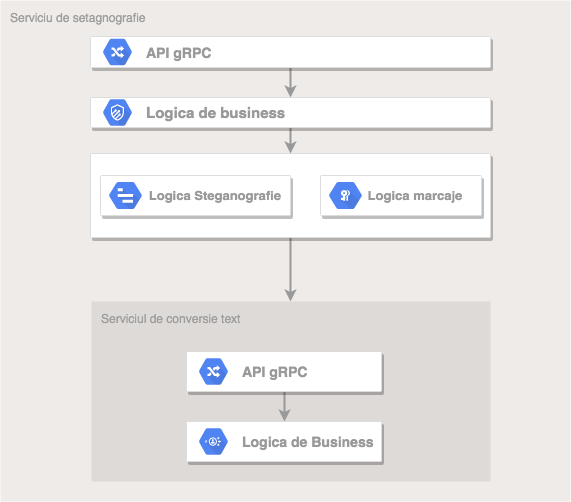
\includegraphics[keepaspectratio=true,scale=0.4]{img/watermarking_arch.png}
\caption{Arhitectura serviciului de marcaje}
\label{water_arch}
\end{center}
\end{figure}

\subsubsection{Aplica'tiile steganografiei}
\subsubsection{Rezultate algoritmi}


\subsection{Microserviciul de compresie} \label{s_compession}
\subsubsection{Introducere}
\subsubsection{Arhitectur'a}

\begin{figure}[H]
\begin{center}
\advance\leftskip-3cm
\advance\rightskip-3cm
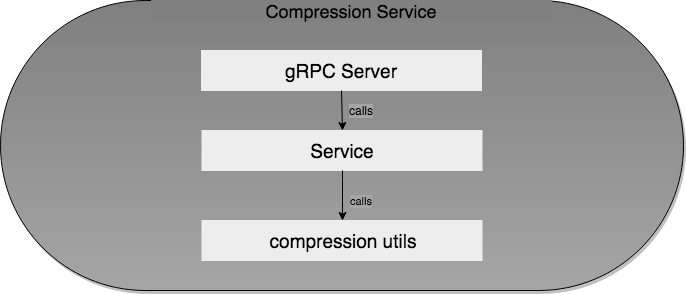
\includegraphics[keepaspectratio=true,scale=0.4]{img/compression_arch.png}
\caption{Arhitectura serviciului de compressie}
\label{compress_arch}
\end{center}
\end{figure}

\subsubsection{Rezultate algoritmi}
Microserviciul de compresie ofer'a 3 func'tionalit'a'ti : compresie text, compresie PNG 'si compresie JPEG.

Compresia de text este bazat'a pe zlib care folose'ste algoritmul DEFLATE, acesta permite utilizarea unui num'ar minim de resurse pentru a ob'tine un rezultat cât mai bun. Algoritmul este unul f'ar'a pierderi.
Rezultatul bun este ob'tinut datorit'a folosirii arborilor de codificare Huffman, deorece se creaz'a un arbore Huffman optimizat pentru fiecare block de date. Totu'si folosirea Huffman este recomandat'a mai mult pentru mesaje mici, deorece aceasta introduce pentru fiecare block ni'stye instruc'tiuni de decompresie.
Compresia este ob'tinut'a prin 2 pa'si:
\begin{enumerate}
\item[•]Potrivirea 'si 'inlocuirea datelor duplicate
\item[•] 'Inlocuirea simbolurilor cu altele noi bazate pe frecven'ta de apari'tie
\end{enumerate}

\begin{small}
\begin{longtable}{|c|c|c|c|c|c|c|} 
\hline               
 \makecell{Dimensiune\\ fi'sier text \\ (octe'ti)} &  \makecell{Tip date}  & \makecell{Dimensiune\\ dup'a\\ compresie \\ (Best)} & \makecell{Dimensiune \\dup'a \\compresie \\ (Default)} & \makecell{Dimensiune \\dup'a \\compresie \\ (Fast)} & \makecell{Dimensiune \\dup'a\\ compresie \\ (Doar Huffman)} & \makecell{Dimensiune \\dup'a\\ compresie \\ (No)} \\ [0.5ex]   
%heading
\hline 
\multirow{2}{*}{99}  & \multirow{2}{*}{Repetat } &  \makecell{ 48 } & \makecell{ 48  }  &  \makecell{ 68 }  & \makecell{ 68  }  & \makecell{ 115 }    \\ & & \fpeval{round(48/99 * 100, 2)}\% & \fpeval{round(48/99* 100, 2)}\% & \fpeval{round(68/99* 100, 2)}\% & \fpeval{round(68/99* 100, 2)}\% & \fpeval{round(115/99* 100, 2)}\% \\
\hline      
99  & Unic  &   \makecell{ 94 \\ \fpeval{round(94/99* 100, 2)}\%}  & \makecell{ 94 \\ \fpeval{round(94/99* 100, 2)}\%} &  \makecell{ 128 \\ \fpeval{round(128/99* 100, 2)}\%} & \makecell{ 94 \\ \fpeval{round(94/99* 100, 2)}\%} &\makecell{ 115 \\ \fpeval{round(115/99* 100, 2)}\%}  \\    
\hline             
      
2022  & Repetat  &   \makecell{ 183 \\ \fpeval{round(183/2022* 100, 2)}\%}  & \makecell{ 183 \\ \fpeval{round(183/2022* 100, 2)}\%} &  \makecell{ 187 \\ \fpeval{round(187/2022* 100, 2)}\%} & \makecell{ 1112 \\ \fpeval{round(1112/2022* 100, 2)}\%}  & \makecell{ 2038 \\ \fpeval{round(2038/2022* 100, 2)}\%}  \\    
 \hline             

1769  & Unic  &  \makecell{ 710 \\ \fpeval{round(710/1769* 100, 2)}\%}  & \makecell{ 710 \\ \fpeval{round(710/1769* 100, 2)}\%} &  \makecell{ 756 \\ \fpeval{round(756/1769* 100, 2)}\%} & \makecell{ 978 \\ \fpeval{round(978/1769* 100, 2)}\%} & \makecell{ 1785 \\ \fpeval{round(1785/1769* 100, 2)}\%}  \\    
  \hline   
  
10240  & Repetat  &   \makecell{ 230 \\ \fpeval{round(230/10240* 100, 2)}\%}  &  \makecell{ 233 \\ \fpeval{round(233/10240* 100, 2)}\%} &   \makecell{ 295 \\ \fpeval{round(295/10240* 100, 2)}\%} &    \makecell{ 5368 \\ \fpeval{round(5368/10240* 100, 2)}\%}  &  \makecell{ 10256 \\ \fpeval{round(10256/10240* 100, 2)}\%}  \\   
\hline             

5277  & Unic  &  \makecell{ 1724 \\ \fpeval{round(1724/5277* 100, 2)}\%}  & \makecell{ 1724 \\ \fpeval{round(1724/5277* 100, 2)}\% } &  \makecell{ 1918 \\ \fpeval{round(1918/5277* 100, 2)}\%} & \makecell{ 2835 \\ \fpeval{round(2835/5277* 100, 2)}\%} & \makecell{ 5293 \\ \fpeval{round(5293/5277* 100, 2)}\%}  \\    

\hline             
  % titlul tabelului
  \caption{Rata de compresie fi'siere text}     
\label{table:textcompressiontable}        

\end{longtable}
\end{small}




\begin{small}
\begin{longtable}{|c|c|c|c|c|}  
\hline               
  &  \makecell{Imagine mic'a}  & \makecell{Imagine medie} & \makecell{Imagine mare} & \makecell{Imagine gigant'a}  \\
%heading
\hline 
\makecell{Dimensiune\\L'a'time x Lungime}& 100 x 120  & 512 x 496 & 1024 x 1500  &  4000 x 4000   \\    
\hline      
      
\makecell{Dimensiune \\(octe'ti)} & \fpeval{ 100 * 120 *3 } &  \fpeval{ 512 * 496 *3 } & \fpeval{ 1024 * 1500 *3 } & \fpeval{ 4000 * 4000 *3 }    \\    
 \hline             

\makecell{Dimensiune\\compresie Best\\ (octe'ti) } & 236 & 1460 & 6646 & 56321  \\   
\hline    

\makecell{Raport dimensiune \\compresie Best } &  \fpeval{ round(236/(100 * 120 *3)*100, 2) } \% & \fpeval{ round(1460/(512 * 496 *3)*100, 2) } \% &  \fpeval{ round(6646/(1024 * 1500 *3)*100, 2) } \% &  \fpeval{ round(56321/(4000 * 4000 *3)*100, 2) } \%  \\   
\hline             
 
 \makecell{Timp execu'tie\\compresie Best (s)}  &  0,025696 & 0,460886617 & 2,69279 &  27,35  \\   
\hline             

\makecell{Dimensiune\\compresie Default\\ (octe'ti) } & 332 & 1825 &  7775 & 56321  \\   
\hline    

\makecell{Raport dimensiune\\compresie Default\\ } &  \fpeval{ round(332/(100 * 120 *3) *100, 2) } \%& \fpeval{ round(1825/(512 * 496 *3)*100, 2) } \% &  \fpeval{ round(7775/(1024 * 1500 *3)*100, 2) } \% &  \fpeval{ round(56321/(4000 * 4000 *3)*100, 2) } \%  \\   
\hline             
 
 \makecell{Timp execu'tie\\compresie Default (s)} & 0,025696 & 0,426049450 & 2,51625 &  26,207 \\   
\hline 

\makecell{Dimensiune\\compresie Fast\\ (octe'ti) } & 333 & 2057 &  9210 & 71688  \\   
\hline    

\makecell{Raport dimensiune\\compresie Fast\\ } & \fpeval{ round(333/(100 * 120 *3)*100, 2) } \% & \fpeval{ round(2057/(512 * 496 *3)*100, 2) } \% & \fpeval{ round(9210/(1024 * 1500 *3)*100, 2) } \% &  \fpeval{ round(71688/(4000 * 4000 *3)*100, 2) } \% \\   
\hline             
 
 \makecell{Timp execu'tie\\compresie Fast (s)} & 0,015916 & 0,270366040 & 1,78344 &  16,9363 \\   
\hline 


\makecell{Dimensiune\\compresie No\\ (octe'ti) } & 36205 & 762756 & 4611603 & 48025301  \\   
\hline    

\makecell{Raport dimensiune\\compresie No\\ } &  \fpeval{ round(36205/(100 * 120 *3)*100, 2) } \% &   \fpeval{ round(762756/(512 * 496 *3)*100, 2) } \% &  \fpeval{ round(4611603/(1024 * 1500 *3)*100, 2) } \% & \fpeval{ round(48025301/(4000 * 4000 *3)*100, 2) } \%  \\   
\hline             
 
 \makecell{Timp execu'tie\\compresie No\\ (secunde) } &0,004395 & 0,047150913 & 0,30246 & 2,97536   \\   
\hline  

  % titlul tabelului
  \caption{Rata de compresie PNG entropie mic'a}

\label{table:pngsmallcompressiontable}             
\end{longtable}
\end{small}

 'In  cazul imaginilor cu o entropie mic'a, de exemplu cele care contin text sau au un procent de fundal foarte mare se ob'tine o rat'a de compresie foarte bun'a cu un factor cuprins 'intre 20 'si 1000. Acest lucru contribuie la sc'aderea pre'tului de stocare per octet, 'ins'a introduce un cost mediu spre mare de timp pentru imaginile foarte mari.
 
 \begin{small}
\begin{longtable}{|c|c|c|c|c|}
\hline               
  &  \makecell{Imagine mic'a}  & \makecell{Imagine medie} & \makecell{Imagine mare} & \makecell{Imagine foarte mare}  \\
%heading
\hline 
\makecell{Dimensiune\\L'a'time x Lungime}& 100 x 120  & 512 x 496 & 1024 x 1500  &  4000 x 4000   \\    
\hline      
      
\makecell{Dimensiune \\(octe'ti)} & \fpeval{ 100 * 120 *3 } &  \fpeval{ 512 * 496 *3 } & \fpeval{ 1024 * 1500 *3 } & \fpeval{ 4000 * 4000 *3 }    \\    
 \hline             

\makecell{Dimensiune\\compresie Best\\ (octe'ti) } & 36215 & 762931& 4612658 & 48036298  \\   
\hline    

\makecell{Raport dimensiune \\compresie Best } &  \fpeval{ round(36215/(100 * 120 *3)*100, 2) } \% &  \fpeval{ round(762931/(512 * 496 *3)*100, 2) } \% & \fpeval{ round(4612658/(1024 * 1500 *3)*100, 2) } \% &   \fpeval{ round(48036298/(4000 * 4000 *3)*100, 2) } \% \\   
\hline             
 
 \makecell{Timp execu'tie\\compresie Best(s)} & 0,055334 & 1,02189 & 5,769 & 65,3939   \\   
\hline             

\makecell{Dimensiune\\compresie Default\\ (octe'ti) } & 36215 & 762931 & 4612658 & 48036298  \\   
\hline    

\makecell{Raport dimensiune\\compresie Default\\ } &  \fpeval{ round(36215/(100 * 120 *3) *100, 2) } \% & \fpeval{ round(762931/(512 * 496 *3)*100, 2) } \%  & \fpeval{ round(4612658/(1024 * 1500 *3)*100, 2) } \% &   \fpeval{ round(48036298/(4000 * 4000 *3)*100, 2) } \% \\   
\hline             
 
 \makecell{Timp execu'tie\\compresie Default (s)} & 0,050935 &  0,989136 & 5,7694 &  62,03826 \\   
\hline 

\makecell{Dimensiune\\compresie Fast\\ (octe'ti) } & 36205 & 762756 & 4611603 &   48025301\\   
\hline    

\makecell{Raport dimensiune\\compresie Fast\\ } & \fpeval{ round(36205/(100 * 120 *3)*100, 2) } \% & \fpeval{ round(762756/(512 * 496 *3)*100, 2) } \%  & \fpeval{ round(4611603 /(1024 * 1500 *3)*100, 2) } \% &   \fpeval{ round(48025301/(4000 * 4000 *3)*100, 2) } \% \\   
\hline             
 
 \makecell{Timp execu'tie\\compresie Fast (s) } & 0,030182 & 0,51095 &  3,0343 & 31,83958   \\   
\hline 


\makecell{Dimensiune\\compresie No\\ (octe'ti)} & 36205 & 762756  & 4611603 &  48025301 \\   
\hline    

\makecell{Raport dimensiune\\compresie No\\ } &  \fpeval{ round(36205/(100 * 120 *3)*100, 2) } \% &  \fpeval{ round(762931/(512 * 496 *3)*100, 2) } \% &  \fpeval{ round(4611603 /(1024 * 1500 *3)*100, 2) } \% &  \fpeval{ round(48025301/(4000 * 4000 *3)*100, 2) } \%  \\   
\hline             
 
 \makecell{Timp execu'tie\\compresie No\\ (secunde) } & 0,004997 & 0,048537 & 0,31703 &  3,02121 \\   
\hline  
\caption{Rata de compresie PNG entropie mare}
  % titlul tabelului
\label{table:pngbigcompressiontable}             
\end{longtable}
\end{small}
'In cazul imaginilor cu o entropie mare compresia cre'ste dimensiunea fi'sierului prin ad'augarea de metadate, iar dimensiunea datelor r'am'ane aceea'si. 'In cazul unor imagini foarte mari de acest tip se poate introduce o 'int'arziere de p'an'a la 35 de secunde f'ar'a a aduce impact asupra pre'tului de stocare. 'Ins'a aceste imagini se 'int'alnesc extrem de rar, aplica'tia ar fi afectat'a foarte pu'tin de acest fenomen.


\subsection{Microserviciul de fisiere} \label{s_file}
\subsubsection{Introducere}
\subsubsection{Arhitectur'a}

\begin{figure}[H]
\begin{center}
\advance\leftskip-3cm
\advance\rightskip-3cm
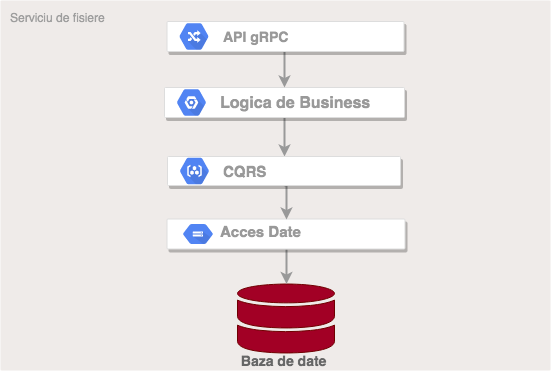
\includegraphics[keepaspectratio=true,scale=0.4]{img/file_arch.png}
\caption{Arhitectura serviciului de fi'siere}
\label{file_arch}
\end{center}
\end{figure}


\subsection{Microserviciul de utilizatori}  \label{s_user}
\subsubsection{Introducere}
\subsubsection{Arhitectur'a}

\begin{figure}[H]
\begin{center}
\advance\leftskip-3cm
\advance\rightskip-3cm
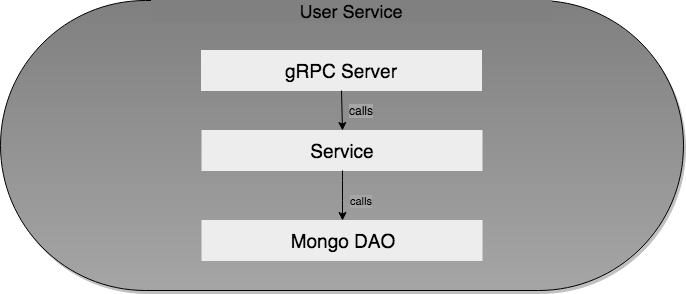
\includegraphics[keepaspectratio=true,scale=0.4]{img/user_arch.png}
\caption{Arhitectura serviciului de utilizatori}
\label{user_arch}
\end{center}
\end{figure}


\section{Arhitectura aplicatiei web}
\subsection{Descriere general'a}
\subsection{Descrierea componentelor}


\chapter{Testare 'si Validare}
Acest capitol con'tine descrierea metodei de testare 'si validate a sistemului. Sunt descrise toolurile care au fost folosite 'si este analizat' procentul de acoperire a codului.

\section{Testarea serverului}
Pentru testarea serverului au fost scrise atât \textit{Unit Teste}, cât 'si \textit{Teste de integrare 'si interac'tiune}. Pentru scrierea 'si executarea testelor au fost folosite 2 \textit{tool}-uri: \textit{testing}, care este integrat 'in limbajul \textbf{Golang}, 'si \textit{testify}, care este o libr'arie \textit{open-source} pentru testare 'in limbajul men'tionat. Pentru o mai bun'a testare, 'inainte de dezvoltarea clientului \textit{web}, s-au efectuat opera'tii de testare utilizând fi'sierele \textit{swagger} create pe baza API-ului serviciilor, 'si utilizând tool-ul \textit{Postman}.

'In teste au fost acoperite toate cazurile de succes 'si majoritatea cazurilor 'in care ar trebui s'a se produc'a o eroare, cum ar fi: parametri invalizi, parametri cu valori eronate sau precondi'tii nesatisf'acute.

\subsection{Reguli de testare 'in Golang}
Pentru ca testele s'a poat'a fi executate automat, numele fiec'arui fi'sier ar trebui s'a contin'a sufixul \textit{\_test}. Fiecare metod'a de test ar trebui s'a 'inceap'a cu prefixul \textit{Test}. 'Indeplinirea acestor condi'tii permite rularea automat'a a testelor 'intr-un mediu de \textit{Dezvoltare continu'a}.

Scrierea unor teste bune nu este un lucru trivial, 'in multe situa'tii sunt foarte multe cazuri de acoperit, ceea ce 'inseamn'a c'atrebuie scrise multe teste, \textbf{Golang} rezolv'a aceast'a problem'a prin ad'augarea de \textit{teste tabelare}, acestea permit crearea testelor imbricate, care pot fi rulate 'in paralel, asfel fiind mai u'sor de detectat \textit{cursele de date}. Acest tip de testare are un avantaj enorm deorece permite scrierea unui cod citibil 'si foarte u'sor de 'in'teles. Fiind integrate 'in limbaj, acest tip de teste pot fi create 'inainte de cod, imadiat dup'a definirea semn'aturilor de metode, ceea ce este ideal pentru o abordare \textit{Test Driven Developement}.

De asemnenea, \textbf{Golang} permiite ad'agarea de func'tii ajut'atoare, a c'aror ordine 'si frecven't'a de rulare poate fi cond'tionat'a, acestea pot fi precondi'tii/postcondi'tii globale sau locale.

\subsection{Testarea serviciilor}

Pentru fiecare serviciu au fost generate un numar de teste egal sau mai mare cu num'arul de metode pe care le are serviciul, in fiecarea test au fost definite seturi tabelare de date pentru a acoperi cât mai multe cazuri. Testele au structura similar'a cu cel reprezentat 'in figura \ref{test_example}.

\begin{figure}[H]
\begin{center}
\advance\leftskip-3cm
\advance\rightskip-3cm
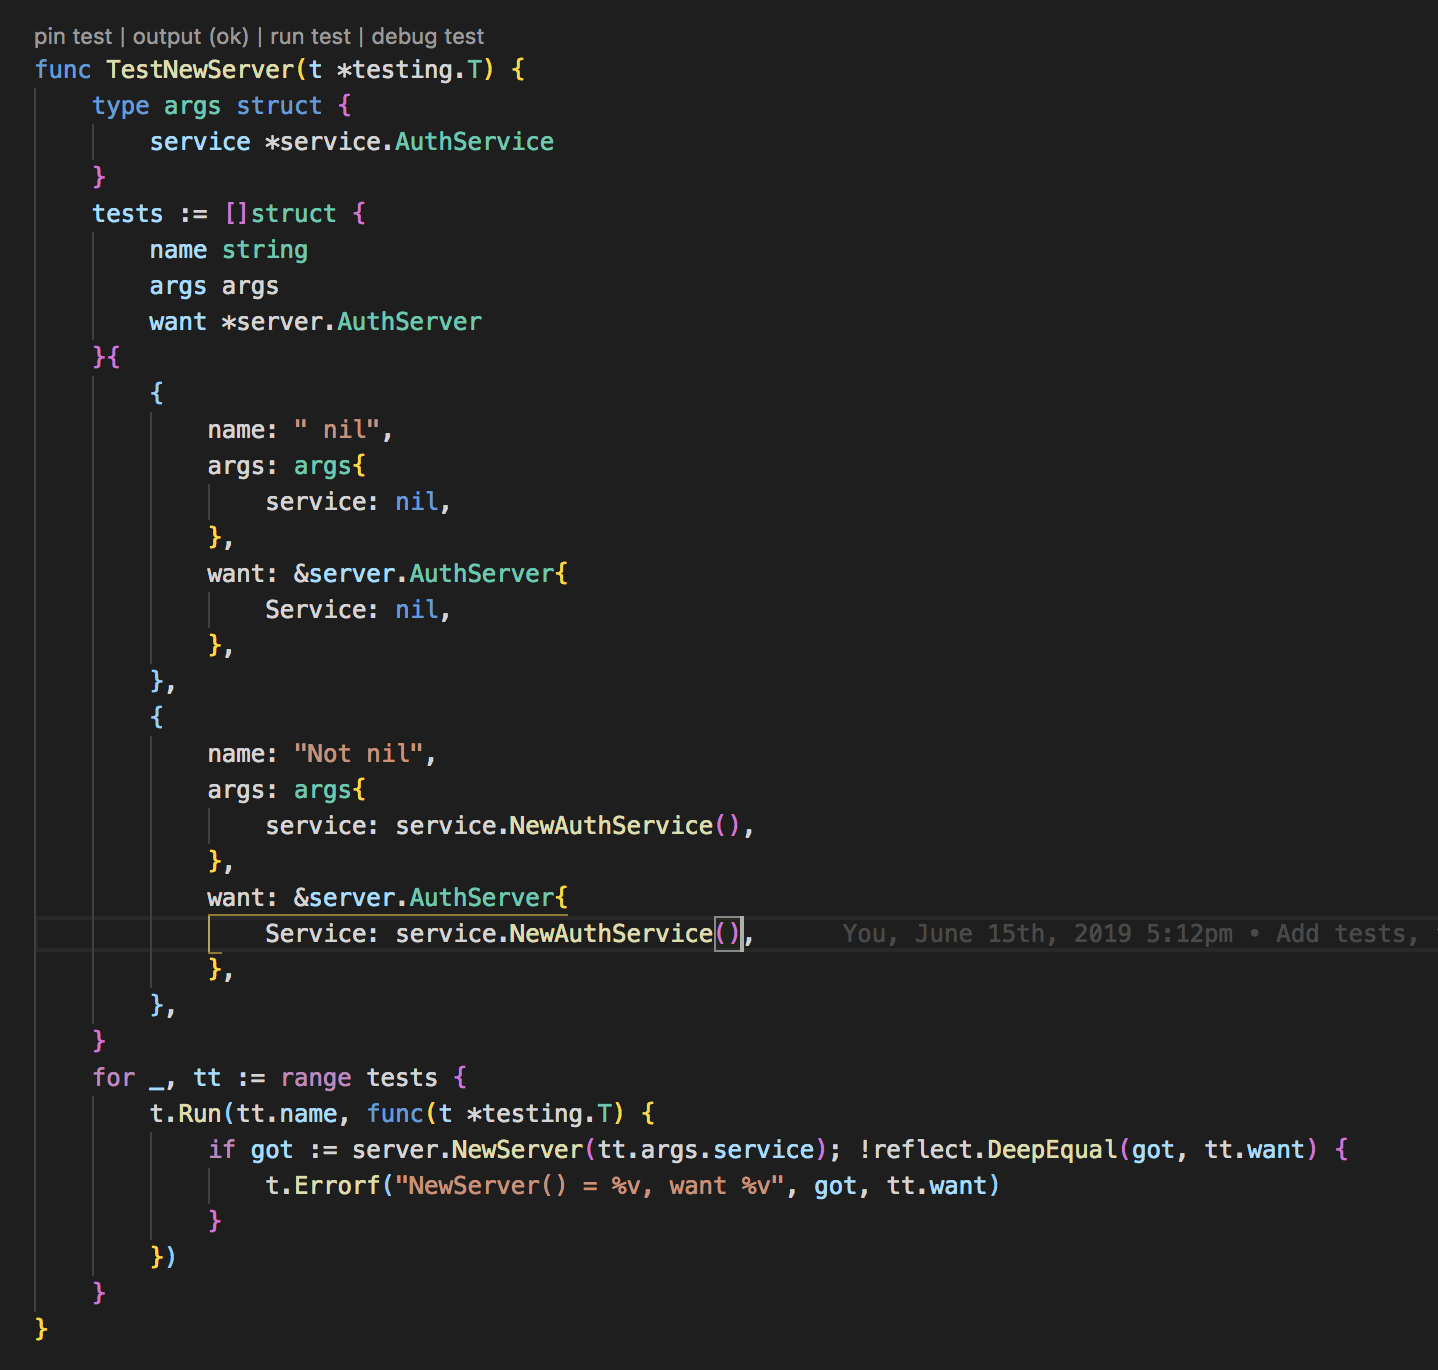
\includegraphics[keepaspectratio=true,scale=0.28]{img/tabel_test.png}
\caption{Exemplu Test}
\label{test_example}
\end{center}
\end{figure}

Rata de acoperire a codului a fost m'asurat'a cu ajutorul unui \textit{tool} care este integrat 'in limbaj, aceasta se nume'ste \textbf{GoCover}. 'In tabelul \ref{table:coverage} este reprezentat'a rata de aceprire cu teste a fiec'arui serviciiu 'in  parte, unele p'ar'ti nu au putut fi acoperite, acestea con'tinând trat'ari de erori care vin din alte libr'arii folosite, o situa'tie de apari'tie a acestora nu a putut fi simulat'a.

\begin{table}[H]
\caption{Rata de acoperire a testelor}
\begin{tabular}{|c|c|c|c|}          
\hline                     
Nume serviciu & Acoperire server(\%) & Acoperire service (\%) & Acoperire altele(\%)   \\ [0.5ex]   
\hline
                              
\end{tabular}
  % titlul tabelului
\label{table:coverage}             
\end{table}


Testarea adecvat'a a avut un rol semnificativ 'in procesul de detec'tie de erori sau comportament nea'steptat. Datorit'a test'arii au fost detectate probleme triviale de securitate, care puteau compromite identitatea 'si datele utilizatorului.


\section{Testarea clientului}
postman si testtare manuala fe
\chapter{Manual de Instalare 'si Utilizare}

\section{Cerin'te preliminare}
\section{Instalare si configurare}

\chapter{Concluzii}


\section{Contribu'tii 'si rezultate ob'tinute}
Aplica'tia ob'tinut'a ofer'a func'tionalit'a'ti de 'inc'arcare 'si desc'arcare  a fi'sierelor, acesta fiind un sistem cu zero cuno'tin'te despre datele stocate 'in sistem, un atacator nu poate s'a pun'a mâna pe datele utilizatorului 'in lipsa parolei de decriptare, aceasta nefiind stocat'a 'in sistem.

Prin ad'augarea compresiei fi'sierelor text 'si a imaginilor, implementate de mine,  am obtinut reducerea coinsiderabil'a a spa'tiului de stocare 'in cazul fi'sierelor mari. De asemnea ad'augarea compresiei a contribuit la cre'sterea securit'a'tii aplica'tiei prin cre'stere nivelului de complexitate pentru decriptare. 


\section{Dezvolt'ari ulterioare}

Opera'tiile de criptare 'si compresie sunt foarte costisitoare 'in cazul unor date mari ca volum 'si cu rat'a de repetare mic'a, o solu'tie care ar eficientiza procesul ar fi combinarea celor 2 opera'tii 'in una singur'a. Acest efect se poate ob'tine prin ad'augarea unor permuta'tii pseudoaleatore 'in procesul de compresie al datelor\cite{comp_crypto}.

Se pot eficientiza func'tionalit'a'tile de 'inc'arcare 'si desc'arcare a datelor prin ad'augarea opera'tiei de desp'ar'tire 'in blocuri, acestea fiind transmise alternativ, opera'tiile de transfer prin re'tea sunt cunoscute a fi cele mai 'incete opera'tii de manipulare a datelor. O astfel de abordare ar putea reduce extrem de mult opera'tiile de transmisie, dar 'si cele de criptare 'si compresie, datorit'a faptului c'a opera'tiile pe blocuri ar putea fi efectuate 'in paralel, 'in loc de serial.


%\addcontentsline {toc}{chapter}{Bibliography} 
\bibliographystyle{IEEEtran} 
\bibliography{thesis}%same file name as for .bib

\definecolor{darkbrown}{rgb}{0.59, 0.29, 0.0}
\definecolor{celestialblue}{rgb}{0.29, 0.59, 0.82}
\definecolor{deepchampagne}{rgb}{0.98, 0.84, 0.65}
\definecolor{munsell}{rgb}{0.0, 0.66, 0.47}

\appendix
\chapter{Sec'tiuni relevante din cod}\label{sectiuni_cod}

\subsubsection{Exemplu de fi'sier \textit{protobuf}}
\begin{tcolorbox}\label{proto_definition}
\scriptsize{
\begin{Verbatim}[commandchars=\\\{\}]

\textcolor{blue}{syntax} = \textcolor{darkbrown}{"proto3"};

\textcolor{blue}{package} \textcolor{darkbrown}{compression_service};
\textcolor{blue}{option} go_package=\textcolor{darkbrown}{"pb"};

\textcolor{blue}{import} \textcolor{darkbrown}{"google/api/annotations.proto"};

\textcolor{blue}{service} \textcolor{munsell}{Compression} \{
    \textcolor{blue}{rpc} \textcolor{deepchampagne}{CompressImage}(\textcolor{munsell}{CompressImageRequest})
                              \textcolor{blue}{returns} (\textcolor{munsell}{CompressImageResponse}) \{
         \textcolor{blue}{option} (google.api.http) = \{
             \textcolor{celestialblue}{get}: \textcolor{darkbrown}{"/compression/api/v1/image/compress"}
        \};
    \}
     \textcolor{blue}{rpc} \textcolor{deepchampagne}{DecompressImage}(\textcolor{munsell}{DecompressImageRequest})
                             \textcolor{blue}{returns} (\textcolor{munsell}{DecompressImageResponse}) \{
         \textcolor{blue}{option} (google.api.http) = \{
            \textcolor{celestialblue}{get}: \textcolor{darkbrown}{"/compression/api/v1/image/decompress"}
       \};
    \}
     \textcolor{blue}{rpc} \textcolor{deepchampagne}{CompressText}(\textcolor{munsell}{CompressTextRequest})
                              \textcolor{blue}{returns} (\textcolor{munsell}{CompressTextResponse}) \{
         \textcolor{blue}{option} (google.api.http) = \{
             \textcolor{celestialblue}{get}: \textcolor{darkbrown}{"/compression/api/v1/text/compress"}
        \};
    \}
     \textcolor{blue}{rpc} \textcolor{deepchampagne}{DecompressText}(\textcolor{munsell}{DecompressTextRequest}) 
                            \textcolor{blue}{returns} (\textcolor{munsell}{DecompressTextResponse}) \{
         \textcolor{blue}{option} (google.api.http) = \{
             \textcolor{celestialblue}{get}: \textcolor{darkbrown}{"/compression/api/v1/text/decompress"}
        \};
    \}
\}

\textcolor{blue}{enum} \textcolor{munsell}{ImageType} \{
	PNG  = 0;
	JPEG = 1;
\}
\textcolor{blue}{message} \textcolor{munsell}{CompressImageRequest} \{
    \textcolor{blue}{bytes} \textcolor{celestialblue}{image} = 1;
\}
\textcolor{blue}{message}\textcolor{munsell}{CompressImageResponse} \{
    \textcolor{blue}{bytes} \textcolor{celestialblue}{image} = 1;
\}
\textcolor{blue}{message} \textcolor{munsell}{DecompressImageRequest} \{
    \textcolor{blue}{bytes} \textcolor{celestialblue}{image} = 1;
\}
\textcolor{blue}{message} \textcolor{munsell}{DecompressImageResponse} \{
    \textcolor{blue}{bytes} \textcolor{celestialblue}{image} = 1;
\}
\textcolor{blue}{message} \textcolor{munsell}{CompressTextRequest} \{
    \textcolor{blue}{bytes} \textcolor{celestialblue}{text} = 1;
\}
\textcolor{blue}{message} \textcolor{munsell}{CompressTextResponse} \{
    \textcolor{blue}{bytes} \textcolor{celestialblue}{text} = 1;
\}
\textcolor{blue}{message} \textcolor{munsell}{DecompressTextRequest} \{
    \textcolor{blue}{bytes} \textcolor{celestialblue}{text} = 1;
\}
\textcolor{blue}{message} \textcolor{munsell}{DecompressTextResponse} \{
    \textcolor{blue}{bytes} \textcolor{celestialblue}{text} = 1;
\}

\end{Verbatim}
}
\end{tcolorbox}


\listoffigures

\listoftables

\chapter{Diagrame UML}

\chapter{Glosar}
\begin{center}
\begin{table}[H]
\centering
\begin{tabu} to 0.8\textwidth { | X[c] | X[c] |  }
 \hline
 Termen     & Defini'tie\\
 \hline
 HTTPS   & \textit{Hyper Text Transfer Protocol Secure} - este o versiune securizat'a a protocolului de transmisie HTTP.  \\
 \hline
 gRPC &  \textit{Google Remote Procedure Call} - framework pentru comunicare 'intre servicii, utilizând protocolul HTTP/2. \\
 \hline
  e2e &  \\
  gRPC &  \\
 HTML &  \\
 framework  &  \\
 DOM &  \\
  RPC &  \\
  Protocol buffers &  \\
 \hline
 
\end{tabu}
\end{table}
\end{center}



\end{document}
